\documentclass{article}

\usepackage{amsthm, amsmath, amssymb} 
\usepackage{authblk}
\usepackage{array}
\usepackage{adjustbox}
\usepackage[backend=biber, style=alphabetic, sorting=ynt]{biblatex}
\usepackage{graphicx}
\usepackage{hyperref}
\usepackage[utf8]{inputenc}
\usepackage{quiver}
\usepackage{listings}
\usepackage{listingsutf8}
\usepackage{tikz-cd}
\usepackage{pgfgantt}
\usepackage{comment}
\usepackage{siunitx}
\usepackage{placeins}
\usepackage{textcomp}
\usepackage{stmaryrd}
\usepackage{color}
\usepackage{thmtools}
\usepackage{fancyhdr}

\DeclareFixedFont{\ttb}{T1}{txtt}{bx}{n}{8}
\DeclareFixedFont{\ttm}{T1}{txtt}{m}{n}{8}

\definecolor{deepblue}{rgb}{0, 0, 0.5}
\definecolor{deepred}{rgb}{0.6, 0, 0}
\definecolor{deepgreen}{rgb}{0, 0.5, 0}

\newcommand\pythonstyle{\lstset{
    language = Python,
    basicstyle = \ttm,
    morekeywords = {self},
    keywordstyle = \ttb\color{deepblue},
    emph={MyClass, __init__},
    numbers = left,
    numberstyle = \tiny\color{gray},
    frame = single, 
    emphstyle = \ttb\color{deepred},
    stringstyle = \color{deepgreen},
    showstringspaces = false
}}

\lstnewenvironment{python}[1][]
{
    \pythonstyle
    \lstset{#1}
}{}

\newcommand\pythonexternal[2][]{{
    \pythonstyle
    \lstinputlisting[#1]{#2}
}}

\newcommand\pythoninline[1]{{\pythonstyle\lstinline!#1!}}

\newcommand\pseudostyle{\lstset{
    language=,
    basicstyle = \ttfamily,
    keywordstyle = \bfseries\color{blue},
    emph = {function, if, then, else, while, for, return, begin, end},
    emphstyle = \bfseries\color{red},
    numbers = left,
    numberstyle = \tiny\color{gray},
    frame = single,
    stringstyle = \color{green},
    showstringspaces = false
}}

\lstnewenvironment{pseudo}[1][]
{
    \pseudostyle
    \lstset{#1}
}{}

\newcommand\cppstyle{\lstset{
    language = C++,
    basicstyle = \ttfamily,
    morekeywords = {class, public, private, protected, virtual, override, final, noexcept, constexpr},
    keywordstyle = \bfseries\color{blue},
    emph = {MyClass, main},
    emphstyle = \bfseries\color{red},
    stringstyle = \color{green},
    commentstyle = \color{gray},
    showstringspaces = false,
    numbers = left,
    numberstyle = \tiny\color{gray},
    frame = single,
    tabsize = 3,
    breaklines = true
}}

\lstnewenvironment{cpp}[1][]
{
    \cppstyle
    \lstset{#1}
}
{}

\newcommand\cppexternal[2][]{{
    \cppstyle
    \lstinputlisting[#1]{#2}
}}

\newcommand\cppinline[1]{{\cppstyle\lstinline!#1!}}

\addbibresource{bibliography.bib}

\declaretheoremstyle[
    headfont = \bfseries, 
    notebraces = {}{},
    headformat = Preuve : \NOTE,
    bodyfont = \normalfont\itshape,
    headpunct = {},
    spacebelow = \parsep,
    spaceabove = \parsep,
    qed = \qedsymbol
]{proofstyle}

\newtheorem{proposition}{Proposition}
\newtheorem{definition}{Définition}
\newtheorem{exemple}{Exemple}
\declaretheorem[name=demo, numbered=yes, style=proofstyle]{preuve}

\lstset{
    inputencoding=utf8,
    extendedchars=true,
    literate=%
    {é}{{\'e}}{1}%
    {è}{{\`e}}{1}%
    {à}{{\`a}}{1}%
    {ç}{{\c{c}}}{1}%
    {œ}{{\oe}}{1}%
    {ù}{{\`u}}{1}%
    {É}{{\'E}}{1}%
    {È}{{\`E}}{1}%
    {À}{{\`A}}{1}%
    {Ç}{{\c{C}}}{1}%
    {Œ}{{\OE}}{1}%
    {Ê}{{\^E}}{1}%
    {ê}{{\^e}}{1}%
    {î}{{\^i}}{1}%
    {ô}{{\^o}}{1}%
    {û}{{\^u}}{1}%
    {ë}{{\¨{e}}}1
    {û}{{\^{u}}}1
    {â}{{\^{a}}}1
    {Â}{{\^{A}}}1
    {Î}{{\^{I}}}1
}

\renewcommand{\contentsname}{Table des matières}

\graphicspath{{./Images}}

\pagestyle{fancy}
\AtEndDocument{\label{lastpage}}
\fancyhead[L]{Mattéo Mennesson et Lucas Noirot}\fancyhead[C]{}\fancyhead[R]{Université de Montpellier}
\fancyfoot[C]{\begin{tabular}{cc} Exploration des Codes de Gray et des Codes de Beckett-Gray \\ \textbf{Page \thepage/\pageref{lastpage}} \\ \end{tabular}}

\renewcommand{\footrulewidth}{0.4pt}

\begin{document}

\begin{figure}
    \centering
    \includegraphics[width=5cm,height=5cm]{logo_univ_mtp.png}\\
\end{figure}

\begin{center}
    {\fontsize{20}{20}\selectfont Université de Montpellier\\}
    {\fontsize{15}{15}\selectfont Faculté des sciences}\\
    {\fontsize{15}{15}\selectfont Place Eugène Bataillon - Campus Triolet – 34090 Montpellier Cedex 5}\\
    {\fontsize{15}{15}\selectfont Année universitaire 2023-2024 }
    \\\
    \\\
    \\\
    
\end{center}

\begin{center}
    \rule{0.8\linewidth}{1pt}
\end{center}

\begin{center}
    \textbf{\\ \huge Exploration des Codes de Gray et des Codes de Beckett-Gray : \Large Implémentation, Heuristiques et Analyses Statistiques dans le Contexte de l'Hypercube} 
    
    \begin{center}
    \rule{0.8\linewidth}{1pt}
    \\\
    \\\
    \\\
    \\\
    \end{center}
\end{center}

\begin{center}
    {\fontsize{15}{15}\selectfont Mémoire de première année du master ALGO}\\
    {\fontsize{15}{15}\selectfont Présenté par Mennesson Mattéo et Noirot Lucas}\\  
    {\fontsize{15}{15}\selectfont Encadré par Stéphane Bessy.}
\end{center}

\newpage

\tableofcontents
\newpage

\section*{Remerciements}
  
Nous tenons à remercier Monsieur Bessy pour son soutien et son enthousiasme tout au long de ce TER. Ses nombreux retours sur la rédaction de notre rapport, ainsi que son aide dans la recherche d'idées pour la partie implémentation, nous ont été très précieux tout au long de notre travail.
\newpage

\section{Introduction}

Les codes de Gray et leurs variantes, tels que les codes de Beckett-Gray, sont un objet d'études passées et récents de la recherche en informatique, en particulier dans le domaine de la théorie de l'information et de la conception des circuits logiques. Leur caractéristique principale réside dans leur capacité à minimiser les transitions binaires entre des mots consécutifs, ce qui les rend particulièrement utiles dans de nombreuses applications, telles que la réduction de la consommation d'énergie dans les circuits électroniques et la transmission de données fiables dans les communications numériques. \newline

Dans ce mémoire, nous nous proposons d'explorer en profondeur les concepts des codes de Gray et des codes de Beckett-Gray, en mettant l'accent sur leur génération et leur utilisation dans le contexte spécifique de l'hypercube. L'hypercube, une structure fondamentale en informatique parallèle et distribuée, offre un cadre idéal pour étudier les propriétés et les performances de ces codes, en raison de sa structure régulière et de ses propriétés topologiques uniques.\newline

Notre travail consistera en trois aspects principaux :
\begin{itemize}
    \item \underline{Implémentation des Codes de Gray et des Codes de Beckett-Gray} : Nous commencerons par présenter des algorithmes de génération de ces codes, en mettant en évidence leurs caractéristiques. Nous développerons ensuite une implémentation efficace de ces algorithmes, en nous appuyant sur des techniques de programmation avancées pour garantir leur performance et leur extensibilité.
    \item \underline{Exploration des Heuristiques} : Dans le but d'améliorer la génération et l'utilisation des codes de Gray et des codes de Beckett-Gray, nous proposerons et évaluerons différentes heuristiques et stratégies d'optimisation. Ces heuristiques visent à identifier et à exploiter les motifs et les régularités présents dans ces codes, afin d'améliorer leur performance.
    \item \underline{Analyses Statistiques et Recherche de Motifs} : Enfin, nous entreprendrons une analyse approfondie des propriétés statistiques des codes de Gray et des codes de Beckett-Gray, en utilisant des outils et des techniques de l'analyse de données. Nous chercherons à identifier des motifs récurrents et des structures sous-jacentes dans ces codes, afin de mieux comprendre leur comportement.
\end{itemize}

En combinant ces trois aspects, notre mémoire vise à fournir de nouvelles perspectives sur les codes de Gray et les codes de Beckett-Gray. Nous espérons que nos résultats contribueront à élargir la compréhension de ces concepts fondamentaux et à ouvrir de nouvelles voies de recherche dans ce domaine passionnant.

\newpage

\section{Organisation du travail}

Nous avons commencé à travailler sur le TER à la fin du mois de janvier, initialement en groupe de quatre personnes. Notre première tâche a été de lire et de nous approprier l'article de Torsten Mütze \cite{CGC}. Ensuite, nous avons développé des codes en JavaScript pour générer des codes de Gray de différents types. Le choix de JavaScript s'explique par la possibilité de visualiser ces codes sur une page web. Par la suite, il nous a été demandé de choisir un problème non résolu de l'article. Nous avons opté pour celui concernant les codes de Beckett-Gray et commencé notre rapport en \LaTeX. Nous nous sommes documentés avec \cite{BGC_fast} et \cite{BGC}. \\

Vers la sixième semaine de travail, deux membres ont quitté notre groupe, nous laissant à deux pour nous répartir les tâches. À ce moment-là, Lucas s'est principalement concentré sur la rédaction du rapport tandis que Mattéo s'occupait du codage. Une problématique de notre TER était de développer des heuristiques. Pour le codage, nous avons abandonné JavaScript au profit de Python, un langage que nous maîtrisons mieux. Cependant, une fois les codes fonctionnels obtenus, nous avons décidé de les transcrire en C\texttt{++} pour améliorer les temps d'exécution, délaissant également Python pour ces tâches, bien qu'il reste utilisé pour l'exploitation des résultats. \\

Après cela, Lucas a principalement effectué des analyses statistiques sur les codes de Beckett-Gray pour $n=5$ et  $n=6$ afin de voir si l'on pouvait en déduire des propriétés, tandis que Mattéo a poursuivi l'écriture du rapport. Voici le diagramme de Gantt associé :

\resizebox{!}{200}{
    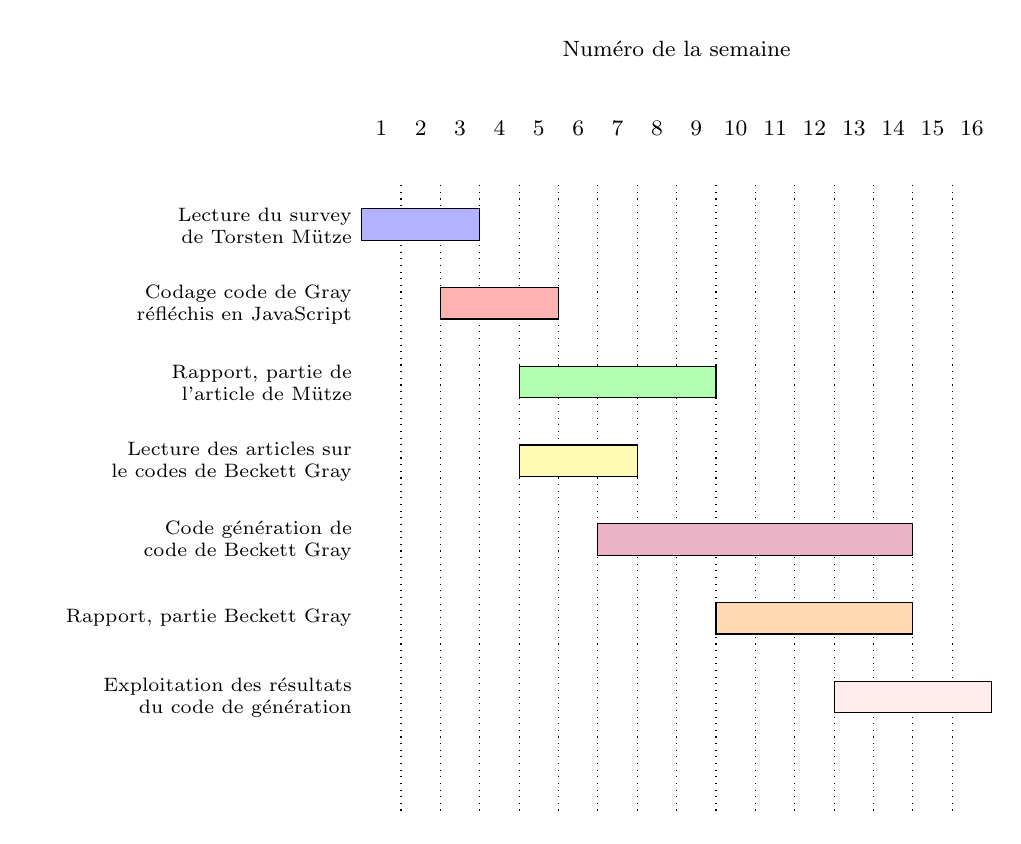
\begin{tikzpicture}
        \centering
        \begin{ganttchart}[
            vgrid, hgrid = {draw = none, draw = none},
            canvas/.append style = {draw = none},
            title/.style = {fill = none},
            milestone label font = \tiny,
            group label font = \tiny,
            title label font = \tiny \footnotesize,
            bar label node/.style = {text width = 4cm, align = right, font = \scriptsize\RaggedLeft, anchor = east},
            milestone label node/.style = {text width = 3cm, align = right, font = \scriptsize\RaggedLeft, anchor = east},
            group label node/.style = {text width = 4cm, align = right, font = \scriptsize\RaggedLeft, anchor = east},
            progress label text = {}
            ]{1}{16},
    
            \gantttitle{Numéro de la semaine}{16} \\
            \gantttitlelist{1,...,16}{1} \\
        
            \ganttbar[bar/.append style={fill=blue!30}]{Lecture du survey de Torsten Mütze}{1}{3} \\
            \ganttbar[bar/.append style={fill=red!30}]{Codage code de Gray réfléchis en JavaScript}{3}{5} \\
            \ganttbar[bar/.append style={fill=green!30}]{Rapport, partie de l'article de Mütze}{5}{9} \\
            \ganttbar[bar/.append style={fill=yellow!30}]{Lecture des articles sur le codes de Beckett Gray}{5}{7} \\
            \ganttbar[bar/.append style={fill=purple!30}]{Code génération de code de Beckett Gray}{7}{14} \\
            \ganttbar[bar/.append style={fill=orange!30}]{Rapport, partie Beckett Gray}{10}{14} \\
            \ganttbar[bar/.append style={fill=pink!30}]{Exploitation des résultats du code de génération}{13}{16} \\

            \end{ganttchart}
    \end{tikzpicture}
}
\newpage

\section{Les codes de Gray.}

Le codage de Gray tient son nom de l'ingénieur américain Frank Gray. Plusieurs codages similaires aux codes de Gray existent, avec des objectifs différents. L'un des objectifs premiers est de générer facilement et rapidement tous les objets d'un ensemble dans un ordre bien précis. Le concept plus généralement connu comme code de Gray combinatoire n'exige plus de coder les nombres mais de lister différents objets d'un ensemble, de sorte que deux objets consécutifs dans la liste diffèrent seulement d'un "petit" changement. Ainsi le codage de Gray est un cas particulier de codage de Gray combinatoire. En informatique, les codes de Gray sont utiles pour minimiser le risque d'erreur pendant la transmission d'une information par exemple, étant donné que pour deux valeurs consécutives, il suffit de changer la valeur d'un seul bit.\newline

Ce code est par exemple utile pour des capteurs de positions absolue, par exemple sur des règles optiques. En effet, si on utilise le code binaire pur, pendant le passage de la position cinq $(101)_2$ à six $(110)_2$ (changement simultané de $2$ bits) il y a un risque de passage transitoire par quatre $(100)_2$ ou sept $(111)_2$, ce que le code Gray évite. Dans un codage de Gray cyclique, le passage du maximum (quinze sur $4$ bits) à zéro se fait également en ne modifiant qu'un seul bit. Ceci permet par exemple d'encoder un angle sur une machine automatique ou un robot.\newline

\begin{definition}
    Un code de Gray est un codage des entiers telle que lorsque on augmente l'entier d'une unité, le codage correspondant ne change que d'un seul bit. Pour le codage binaire tel que l'on le connaît, cette propriété n'est pas respectée, par exemple pour passer de $1$ à $2$, on change deux bits dans leurs représentation binaire, afin de passer de $001$ à $010$.
\end{definition}

\begin{definition}
    Un code de Gray est cyclique quand son premier élément et son dernier élément diffèrent d'un seul bit.
\end{definition}

Le tableau suivant illustre ce qu'est un code de Gray, pour un codage cyclique sur $3$ bits.

{
    \centering
    \begin{tabular}{|c|c|c|} \hline
        Nombre & Codage binaire & Codage de Gray \\ \hline
        $1$ & $001$ & $000$ \\ \hline
        $2$ & $010$ & $001$ \\ \hline
        $3$ & $011$ & $011$ \\ \hline
        $4$ & $100$ & $010$ \\ \hline
        $5$ & $101$ & $110$ \\ \hline
        $6$ & $110$ & $111$ \\ \hline
        $7$ & $111$ & $101$ \\ \hline
\end{tabular} \par}

\subsection{Construction}
On peut construire récursivement un code de Gray de la manière suivante, cette construction est aussi appelée code binaire réfléchi.

$$L_0 = \epsilon$$
$$L_n = 0L_{n-1}, 1\overline{L_{n-1}}$$

où on a $\Sigma = \{0, 1\}$, $\epsilon$ représente le mot vide $aL_n$ représente la concaténation entre $a$ et $L_n$, avec $a \in \{0, 1\}$ et $\overline{L}$ la réversion de $L$ (le premier élément de L devient le dernier élément de $L$, le deuxième élément de $L$ devient l'avant dernier élément de $L$, etc $\cdots$). Par exemple $\overline{abcd} = dcba$. On remarque le parallèle entre cette construction récursive et la construction récursive dans les hypercubes.\\


Par exemple, voici les premières valeurs des listes $L_1$, $L_2$ et $L_3$.

$$L_1 = 0,1$$
$$L_2 = 00, 01, 11, 10$$
$$L_3 = 000, 001, 011, 010, 110, 111, 101, 100$$
Ainsi, un codage de Gray suivant cette méthode récursive existe toujours.

\subsection{Implémentation}
Dans cette sous-section, on présente différentes implémentations d'algorithmes générant des codes de Beckett-Gray. Les codes utilisés sont disponibles sur \href{https://github.com/Crowreed/GrayCodeCollection}{github}.

\subsubsection{GC}
\begin{python}
    def GC(n):
        if n==1:
            return [0, 1]
        
        l=[0]*(2**n)
    
        for i in range (2**(n-1)):
            l[i] = [0]+[GC(n-1)[i]]
        for i in range (2**(n-1), 2**n):
            l[i] = [1]+[list(reversed(GC(n-1)))[i-2**(n-1)]]

        for i in range (2**n):
            l[i]=flatten_list(l[i])
        return l
\end{python}

Ce code est une implémentation de l'algorithme de génération de séquences de Gray réfléchie. \\ 

La fonction $GC(n)$ prend un entier $n$ comme argument et génère une séquence de Gray de longueur $2^n$, sur des chaînes binaires de longueur $n$. La condition if $n==1$: renvoie $[0, 1]$, qui est la séquence de Gray pour $n=1$. Ensuite, un tableau $l$ est initialisé avec des zéros, de longueur $2^n$. Deux boucles for sont utilisées pour remplir la première moitié et la deuxième moitié du tableau $l$ avec des sous-listes correspondant à la génération récursive des séquences de Gray pour $n-1$. La fonction flatten\_list est utilisée pour aplatir les sous-listes. La séquence résultante est renvoyée. La récursivité de cet algorithme entraîne une utilisation importante de la mémoire pour de grandes valeurs de $n$. \newline

\subsubsection{GCParity}

\begin{python}
    def GCParity(n):
        l = [[0]*n]
        for i in range(1,2**n):
            if (i%2)==1:
                l.append(l[-1].copy())
                l[-1][-1]=l[-1][-1]^1
            else:
                for k in range(n-1,-1,-1):
                    if l[-1][k]==1:
                        l.append(l[-1].copy())
                        l[-1][k-1]=l[-1][k-1]^1
                        break
        return l
\end{python}

C'est une autre façon de générer une séquence de Gray. Cela fonctionne en regardant la parité de l'indice de la ligne du code que l'on génère. Si cette ligne est impaire, il suffit juste d'inverser le dernier bit de la ligne précédente, ici réalisé avec un XOR entre ce bit et $1$. Si cette ligne est paire, on inverse le bit juste à gauche du bit à $1$ le plus à droite.

\subsubsection{GCmod}

\begin{python}
    def GCmod(n):
    l = [[0]*n for i in range(2**n)]
    for i in range(2**n):
        for j in range(n):
            if (i+2**j+2**(j+1))%(2**(j+2)) < 2**(j+1):
                l[i][n-j-1] = 1
    return l
\end{python}
Une dernière façon de générer une séquence de Gray. On cherche à trouver où rajouter les $1$ dans la séquence en utilisant le fait que les bits à la position $j$ sont changés tous les $2^{j+1}$ itérations.\\

\begin{table}[h!]
    \centering
    \caption{Représentation graphique d'un code de Gray $n=5$}
    \vspace{0.5cm}
    \includegraphics[scale=0.2]{exemple.png}
\end{table}
\FloatBarrier

On peut l'observer sur cette représentation graphique un code de Gray pour $n=5$, où les bits au centre changent toutes les deux itération, puis ceux à côté en allant vers l'extérieur toutes les quatre itérations, puis toutes les huit itérations etc.

\subsection{Graphe de retournement}

Le graphe de retournement est un concept utilisé dans le domaine des codes de Gray et des problèmes combinatoires. Ce graphe est utilisé pour représenter les relations entre les objets combinatoires qui sont générés ou répertoriés par un code de Gray. On appellera parfois retournement par flip, la notation anglaise. \newline

Dans un graphe de retournement, chaque sommet représente un objet combinatoire, comme une séquence de $n$-bits dans le cas des codes de Gray sur des mots binaires de tailles $n$. Deux sommets sont reliés par une arête si les objets correspondants diffèrent par une petite modification, souvent appelée "retournement", ce retournement correspond à une distance qui est appelée distance de Hamming et est souvent égale à $1$. Par exemple, dans le contexte des codes de Gray, un retournement peut être l'inversion d'un seul bit dans la séquence. Si le retournement est une opération réversible, c'est-à-dire qu'elle ramène l'objet initial à son état d'origine lorsqu'elle est appliquée deux fois, le graphe de retournement est non dirigé. Un graphe de retournement offre une représentation visuelle des relations entre les objets combinatoires générés par un code de Gray, ce qui facilite l'analyse et la compréhension des propriétés et des comportements de ces codes. \newline

Voici par exemple le graphe de retournement des sous-ensemble de $\{1, 2, 3, 4, 5\}$ de taille $2$, aussi connu sous le nom de graphe de Kneser pour $n=5$ et $k=2$, aussi noté $K(5, 2)$, deux sommets sont voisins si ils sont disjoints.

{
\centering
\begin{center}
    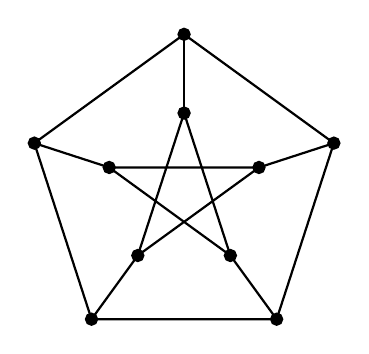
\begin{tikzpicture}[style=thick]
        \draw (18:2cm) -- (90:2cm) -- (162:2cm) -- (234:2cm) -- (306:2cm) -- cycle;
        \draw (18:1cm) -- (162:1cm) -- (306:1cm) -- (90:1cm) -- (234:1cm) -- cycle;
        \foreach \x in {18,90,162,234,306}{
            \draw[fill=black] (\x:2cm) circle (2pt);
            \draw[fill=black] (\x:1cm) circle (2pt);
        }
        \foreach \x in {18,90,162,234,306}{
            \draw (\x:1cm) -- (\x:2cm);
        }
    \end{tikzpicture}
\end{center}
\par
}

Le graphe de retournement associé au code de Gray pour une distance de Hamming de $1$ correspond à l'hypercube $\mathcal{Q}_n$, une structure topologique importante en informatique parallèle et distribuée. Ainsi, les propriétés du graphe de retournement fournissent des informations précieuses sur les relations entre les éléments du code de Gray et sur la structure de l'hypercube.\newline

\subsection{Étude de l'hypercube}
Dans cette partie, on va s'intéresser à étudier en détail l'hypercube, objet central de notre mémoire. Cette partie repose sur l'article wikipedia de l'hypercube \cite{hyp_1} et sur l'article qui résume l'état actuel des connaissances en informatique sur l'hypercube \cite{hyp_2}. L'hypercube est un graphe beaucoup étudié de part son utilité en informatique, que ce soit le parallélisme ou bien les codes de Gray. \\

\begin{definition}
    Un code de Gray correspond à un chemin Hamiltonien sur $\mathcal{Q}_n$ vu comme un graphe de retournement
\end{definition}

\begin{definition}
    Un code de Gray cyclique correspond à un cycle hamiltonien sur l'hypercube $\mathcal{Q}_n$ vu comme un graphe de retournement. Il y a une correspondance bijective.
\end{definition}

Grâce à cette correspondance avec les graphes, l'analyse des codes de Gray devient une analyse de chemin hamiltonien, plus accessible. Nous allons particulièrement nous pencher sur les opérations qui préservent l'intégrité des codes de Gray.

On s'intéresse à l'hypercube $\mathcal{Q}_n$ de dimension $n$ car c'est une représentation sous forme de graphe des $2^n$ mots possibles, quand on les codes avec $n$ bits. 

\begin{definition}
    On peut construire $\mathcal{Q}_n$ comme le graphe dont les sommets sont les $2^n$ vecteurs booléens $n$-dimensionnel, autrement dit les vecteurs avec des coordonnées binaires, et dont deux sommets sont adjacents si et seulement si les vecteurs ne diffèrent que d'une coordonnée.
\end{definition}

Il est aussi possible de construire récursivement $\mathcal{Q}_n$ à partir de deux copies de $\mathcal{Q}_{n-1}$.

\begin{definition}
    Soient deux graphes $G=(V,E)$ et $G'=(V',E')$. Le produit cartésien $H = G \times G'$ est défini comme suit :
    \begin{itemize}
        \item $V(H)=\{(s,s')~|~s\in V,~ s' \in V'\}$ 
        \item $E(H)=\{e_{\{(u,u'),(v,v')\}}|~( u =v \wedge (u'v'\in E')) \vee (u'=v' \wedge (uv\in E))\}$.
    \end{itemize}
\end{definition}

\begin{definition}
    Le $n$-cube, ou l'hypercube de dimension $n$ noté $\mathcal{Q}_n$ est défini récursivement comme le produit cartésien de deux graphes :
    $$\mathcal{Q}_1 = K_2$$
    $$\mathcal{Q}_n = K_2 \times \mathcal{Q}_{n-1}$$
\end{definition}

\begin{table}[h!]
    \centering
    \begin{tabular}{c}
        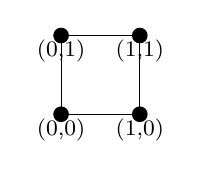
\begin{tikzpicture}
            \foreach \x in {0,1} {
                \foreach \y in {0,1} {
                    \node at (\x, \y) [circle, fill, inner sep=2pt] {};
                    \node at (\x, \y-0.2) {\footnotesize (\x,\y)};
                }
            }
            \draw (0,0) -- (1,0);
            \draw (1,0) -- (1,1);
            \draw (1,1) -- (0,1);
            \draw (0,1) -- (0,0);
        \end{tikzpicture}
        
        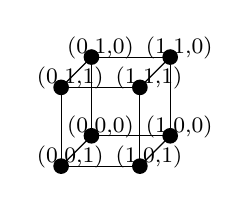
\begin{tikzpicture}
            \foreach \x in {0,1} {
                \foreach \y in {0,1} {
                    \foreach \z in {0,1} {
                        \node at (\x, \y, \z) [circle, fill, inner sep=2pt] {};
                        \node at (\x, \y, \z-0.3) {\footnotesize (\x,\y,\z)};
                    }
                }
            }
            \foreach \x in {0,1} {
                \foreach \y in {0,1} {
                    \draw (\x, \y, 0) -- (\x, \y, 1);
                }
            }
            \foreach \x in {0,1} {
                \foreach \z in {0,1} {
                    \draw (\x, 0, \z) -- (\x, 1, \z);
                }
            }
            \foreach \y in {0,1} {
                \foreach \z in {0,1} {
                    \draw (0, \y, \z) -- (1, \y, \z);
                }
            }
        \end{tikzpicture}
    \end{tabular}
    \caption{Figure représentant $\mathcal{Q}_2$ et $\mathcal{Q}_3$}
    \label{tab:my_label}
\end{table}
\FloatBarrier

On rappelle les notations qu'un graphe $G=(V, E)$ a $p = |V|$ sommets et $q = |E|$ arêtes, on dit qu'il est d'ordre $p$ et de taille $q$. Ainsi, $\mathcal{Q}_n$ est d'ordre $2^n$ et de taille $n 2^{n-1}$. \\

On parle de distance, notée $d$, dans un graphe comme le nombre de coordonnées dans lesquels deux vecteurs booléens diffèrent, par exemple dans $\mathcal{Q}_3$, $d(001, 111) = 2$. Si on considère le graphe comme un graphe de retournement, on parle de distance de Hamming.

\begin{proposition}
    Le diamètre de $\mathcal{Q}_n$ est $n$, on rappelle que le diamètre est la plus grande distance entre deux paires de sommets.
\end{proposition}

\begin{proposition}
    La somme de toutes les distances entre deux paires de sommets dans $Q_n$, notée $T_d$, est égale à $n 2^{2n-2}$.
\end{proposition}

\begin{preuve}
    On note l'ensemble des sommets de $\mathcal{Q}_n$ par $\{v_1, \cdots, v_p\}$.\\

    On a 
    $$T_d(\mathcal{Q}_n) = \underset{1 \leq i < j \leq p}{\sum} d(v_i, v_j)$$

    On partitionne maintenant $\mathcal{Q}_n$ en deux sous-hypercube $\mathcal{Q}_{n-1}$ et $\mathcal{Q}_{n-1}'$. Soit $v_i$ un sommet de $\mathcal{Q}_{n-1}$ et $v_i'$ un voisin de $v_i$ dans $\mathcal{Q}_{n-1}'$. On a la distance de $v_i$ à tous les sommets de $\mathcal{Q}_n$ qui est égale à

    $$T_{d_i}(\mathcal{Q}_n) := \underset{j}{\sum} d(v_i, v_j)$$

    Maintenant, la distance totale de $v_i$ à tous les sommets de $\mathcal{Q}_{n-1}$ est $T_{d_i}(\mathcal{Q}_{n-1})$ et la distance de $v_i$ à un sommet $v_j'$ de $\mathcal{Q}_{n-1}'$ est $d(v_i', v_j')+1$ car $d(v_i, v_i')=1$.\\

    Ainsi la distance totale de $v_i$ aux $2^{n-1}$ sommets de $\mathcal{Q}_{n-1}'$ est 
    $$\underset{j}{\sum} (d(v_i', v_j') +1)= T_{d_i}(\mathcal{Q}_{n-1}) + 2^{n-1}$$

    Ce qui implique $T_{d_i}(\mathcal{Q}_n)=2T_{d_i}(\mathcal{Q}_{n-1}) +2^{n-1}$. On vérifie par récurrence sur $n \in \mathbb{N}$ que $$T_{d_i}(\mathcal{Q}_n) = n 2^{n-1}$$
    Maintenant $\underset{i}{\sum} T_{d_i}(\mathcal{Q}_n)=2^n T_{d_i}(\mathcal{Q}_n) = 2T_d(\mathcal{Q}_n)$ et finalement,  
    $$T_d(\mathcal{Q}_n) = n 2^{2n-2}$$
\end{preuve}

\begin{proposition}
    La distance moyenne dans $\mathcal{Q}_n$ est $\partial(\mathcal{Q}_n) = \frac{n 2^{n-1}}{2^n-1}$
\end{proposition}

\begin{preuve}
    On divise la somme de toutes les distances par $\binom{p}{2}$ où $p$ est le nombre de sommet du graphe, ici $p = 2^n$.\\

    On a $\binom{2^n}{2} = \frac{(2^n)!}{(2^n-2)!2!} = \frac{(2^n)(2^n-1)(2^n-2)!}{(2^n-2)!2!} =  2^{n-1} \times (2^n-1)$.\\

    Ainsi, $$\partial(\mathcal{Q}_n) = \frac{T_d(Q_n)}{\binom{2^n}{2}} = \frac{n 2^{2n-2}}{2^{n-1} \times (2^n-1)} = \frac{n 2^{n-1}}{2^n-1}$$
\end{preuve}

On remarque que quand $n$ devient grand, ce ratio se rapproche de $\frac{n}{2}$. \newline

\begin{proposition}
    Les assertions suivantes sont équivalentes :
    \begin{itemize}
        \item Pour tout $n \in \mathbb{N}^*$, $\mathcal{Q}_n$ est $2$-coloriable, son nombre chromatique est $2$.
        \item Pour tout $n \in \mathbb{N}^*$, $\mathcal{Q}_n$ ne possède pas de cycles impair.
        \item Pour tout $n \in \mathbb{N}^*$, $\mathcal{Q}_n$ est biparti.
    \end{itemize}
\end{proposition}

Ces assertions sont équivalentes quelque soit le graphe considéré. Ces points peuvent se démontrer en utilisant la construction récursive de $\mathcal{Q}_n$, ou d'un point de vue différent en considérant $\mathcal{Q}_n$ comme un graphe de retournement, étant trivial que ces assertions soient équivalentes, on va juste montrer que $\mathcal{Q}_n$ est biparti.

\begin{preuve}
    Tous les sommets de $\mathcal{Q}_n$ sont de degré $n>0$. Les deux ensembles $A=\{\#1$ dans $v$ est pair $\}$ et $B=\{\#1$ dans $v$ est impair$\}$ forment une bipartition de $\mathcal{Q}_n$. Il est rapide de vérifier que pour $v_1, v_2 \in A$ (resp. $v_1, v_2 \in B$), $d(v_1, v_2) \geq 2$ et donc $v_1v_2$ n'est pas une arête de $\mathcal{Q}_n$. Ce n'est pas un biparti complet.
\end{preuve}

\begin{proposition}
    Pour tout $n \in \mathbb{N}^*$, $\mathcal{Q}_n$ est Hamiltonien.
\end{proposition}

Cette proposition peut se montrer par récurrence sur $n \in \mathbb{N}$ en voyant $\mathcal{Q}_n$ non plus comme un graphe de retournement mais comme la construction récursive de deux hypercubes de dimensions $n-1$.\\

Un code de Gray cyclique est un cycle hamiltonien sur $\mathcal{Q}_n$. Comme $\mathcal{Q}_n$ est hamiltonien, cela signifie que pour tout $n \in \mathbb{N}$, il existe un code de Gray cyclique sur des mots binaires de longueur $n$. \\

En général, $\mathcal{Q}_n$ ne possède pas un seul chemin Hamiltonien, ainsi il n'existe pas un unique codage de Gray pour $n$ fixé. Voici par exemple un tableau donnant le nombre de chemins Hamiltonien en fonction de $n$. On détaillera la notion de cycles isomorphes plus tard.

\begin{table}[h]
    \centering
    \begin{tabular}{|c|c|c|}
    \hline
        n & Sans compter les cycles isomorphes & En comptant tous les cycles\\ \hline
        $2$ & $1$ & $1$ \\ \hline
        $3$ & $1$ &  $6$\\ \hline
        $4$ & $9$ & $1344$\\ \hline
        $5$ & $275065$ & $906~545~760$\\ \hline
    \end{tabular}
    \caption{Nombre de cycle Hamiltoniens}
    \label{tab:my_label}
\end{table}

Pour $n \geq 6$ ces valeurs ne sont pas connues. \newline

Le chemin Hamiltonien de $\mathcal{Q}_1$ et le cycles hamiltoniens de $\mathcal{Q}_2$ et $\mathcal{Q}_3$ sont représenté en rouge.

\begin{table}[!h]
    \begin{tabular}{|p{5cm}|c|} \hline
    Code de Gray associé & Hypercube \\ \hline
    
    $0 \rightarrow 1$  & 
    \begin{tikzcd}
        0 & 1
	    \arrow[no head, from=1-1, to=1-2]
	    \arrow[color={rgb,255:red,214;green,92;blue,92}, curve={height=6pt}, dashed, no head, from=1-1, to=1-2]
    \end{tikzcd} \\ \hline
    
    $00 \rightarrow 10 \rightarrow 11 \rightarrow 01$ & 
    \begin{tikzcd}
	    00 & 10 \\
	    01 & 11
	    \arrow[no head, from=1-1, to=1-2]
	    \arrow[color={rgb,255:red,214;green,92;blue,92}, curve={height=6pt}, dashed, no head, from=1-1, to=1-2]
	    \arrow[no head, from=1-1, to=2-1]
	    \arrow[no head, from=2-1, to=2-2]
	    \arrow[no head, from=2-2, to=1-2]
	    \arrow[color={rgb,255:red,214;green,92;blue,92}, curve={height=6pt}, dashed, no head, from=1-2, to=2-2]
	    \arrow[color={rgb,255:red,214;green,92;blue,92}, curve={height=6pt}, dashed, no head, from=2-2, to=2-1]
	    \arrow[color={rgb,255:red,214;green,92;blue,92}, curve={height=6pt}, dashed, no head, from=2-1, to=1-1]
    \end{tikzcd} \\ \hline
    
    $000 \rightarrow 001 \rightarrow 101 \rightarrow 100 \rightarrow 110 \rightarrow  111 \rightarrow 011 \rightarrow 010$ & 
    \begin{tikzcd}
	    001 &&& 011 \\
	    & 101 & 111 \\
	    & 100 & 110 \\
	    000 &&& 010
	    \arrow[no head, from=2-2, to=2-3] \arrow[no head, from=2-2, to=3-2]
	    \arrow[no head, from=3-2, to=3-3] \arrow[no head, from=3-3, to=2-3]
	    \arrow[color={rgb,255:red,214;green,92;blue,92}, curve={height=6pt}, dashed, no head, from=2-3, to=3-3] \arrow[color={rgb,255:red,214;green,92;blue,92}, curve={height=6pt}, dashed, no head, from=3-3, to=3-2]
	    \arrow[color={rgb,255:red,214;green,92;blue,92}, curve={height=6pt}, dashed, no head, from=3-2, to=2-2] \arrow[no head, from=2-2, to=1-1]
	    \arrow[no head, from=1-1, to=4-1] \arrow[no head, from=4-1, to=3-2]
	    \arrow[no head, from=4-1, to=4-4] \arrow[no head, from=4-4, to=3-3]
	    \arrow[no head, from=2-3, to=1-4] \arrow[no head, from=1-4, to=1-1]
	    \arrow[no head, from=1-4, to=4-4]
	    \arrow[color={rgb,255:red,214;green,92;blue,92}, curve={height=6pt}, dashed, no head, from=2-2, to=1-1]
	    \arrow[color={rgb,255:red,214;green,92;blue,92}, curve={height=6pt}, dashed, no head, from=1-1, to=4-1]
	    \arrow[color={rgb,255:red,214;green,92;blue,92}, curve={height=6pt}, dashed, no head, from=4-1, to=4-4]
	    \arrow[color={rgb,255:red,214;green,92;blue,92}, curve={height=6pt}, dashed, no head, from=4-4, to=1-4]
	    \arrow[color={rgb,255:red,214;green,92;blue,92}, curve={height=6pt}, dashed, no head, from=1-4, to=2-3]
    \end{tikzcd} \\ \hline
    \end{tabular}
    \caption{Un code de Gray sur $n$ bits associé à un cycle Hamiltonien dans $\mathcal{Q}_n$}
    \label{tab:my_label}
\end{table}
\FloatBarrier

Dans ce mémoire, nous allons principalement nous concentrer sur l'analyse de $\mathcal{Q}_5$, étant donné que les codes de Beckett-Gray sont disponibles pour tout $n\geq5$. Nous aborderons brièvement le cas $n=6$, bien que les temps de calcul soient considérablement plus longs dans ce cas. Le diamètre de $\mathcal{Q}_5$ (resp. $\mathcal{Q}_6$ est de $5$ (resp. $6$), son ordre est de $32$ (resp. $64$) et sa taille est de $80$ (resp. $192$), chaque sommet de $\mathcal{Q}_5$ (resp. $\mathcal{Q}_6$) a un degré de $5$ (resp. $6$), une somme totale de toutes les distances égale à $1280$ (resp. $6144$) ainsi qu'une distance moyenne entre deux sommets de $2,58$ (resp. $3,04$).

\subsection{Cycles isomorphes dans l'hypercube vu comme un graphe de retournement}

Une autre notion que nous allons examiner sur l'hypercube $\mathcal{Q}_n$ en le considérant comme un graphe de retournement, concerne les cycles isomorphes. La notion de cycles isomorphes nous amène à la notion de code de Gray isomorphes, c'est donc une notion très utile pour étudier la structure des codes de Gray. Dans toute la suite on suppose $n > 3$. On définit préalablement ce qu'on entends par l'égalité de deux cycles. Deux cycles $c_1$ et $c_2$ sont dis égaux si ils parcourent les mêmes sommets dans le même ordre.

\begin{definition}
    Une permutation de l'ensemble $\{1, \cdots, n\}$ est une bijection de $\{1, \cdots, n\}$ dans $\{1, \cdots, n\}$.
\end{definition}

\begin{definition}
    On appelle groupe symétrique d’indice $n$, noté $\mathcal{G}_n$ l’ensemble des permutations de l’ensemble $\{1, 2, 3, \cdots , n\}$. 
\end{definition}

\begin{definition}
    Une permutation circulaire $\sigma$ de $\{a_1, \cdots, a_k\}$ est définie par $\sigma(a_j) = a_{j+1}$ pour tout $j \in \{1, \cdots,  n-1\}$ et $\sigma(i_n) = \sigma (a_1)$
\end{definition}

Du point de vue informatique, on prend le dernier élément d'une liste, qu'on rajoute au début de la liste. L'inverse d'une permutation circulaire consiste à prendre le premier élément de la liste et le mettre à la fin de cette liste. C'est une involution.

\begin{proposition}
    On a $|\mathcal{G}_n|=n!$.
\end{proposition}

\begin{definition}
    On dit que deux codes de Gray $c_1=(v_1, \cdots, v_n)$ et $c_2=(w_1, \cdots, w_n)$ sont isomorphes si il existe $\sigma \in \mathcal{G}_n$ tel que :

    Pour tout $i \in \{1, \cdots, n\}$, $v_i=\sigma(w_i)$ où $\sigma (w_i)$ désigne la permutation des coordonnées de $w_i$.
\end{definition}

On note $c_1 \simeq c_2$ si $c_1$ est isomorphe à $c_2$. 

\begin{proposition}
    $\simeq$ est une relation d'équivalence.
\end{proposition}

\begin{preuve}
    Il faut montrer que $\simeq$ est réflexive, symétrique et transitive.
    \begin{itemize}
        \item $\simeq$ est \underline{réflexive} : $$c_1 \simeq c_1$$ en revenant à la définition de cycles isomorphes et prenant la permutation identité.
        \item $\simeq$ est \underline{symétrique} : si $c_1 \simeq c_2$ alors $c_2 \simeq c_1$ en revenant à la définition de cycles isomorphes et prenant la permutation inverse.
        \item $\simeq$ est \underline{transitive} : si $c_1 \simeq c_2$ et $c_2 \simeq c_3$ alors $c_1 \simeq c_3$ en revenant à la définition de cycles isomorphes et en prenant la composition des deux permutations.
    \end{itemize}
\end{preuve}

On peut donc parler de classes d'équivalences de cycles isomorphes que l'on notera $eq_c := \{c ~|~ c \simeq a\}$, le choix d'un représentant $c$ est arbitraire.

\begin{proposition}
    Dans $\mathcal{Q}_n$, $\# eq_c = n!$.
\end{proposition}

Si on trouve un cycle hamiltonien sur $\mathcal{Q}_n$ on peut en trouver $n!$ autres cycles hamiltonien. Cela nous donne une borne inférieur du nombre de code de cycles hamiltonien dans $\mathcal{Q}_n$.

\begin{proposition}
    Il y a $\binom{n}{i}$ mots possibles de longueur $n$ sur l'alphabet $\{0,1\}$ qui possède $i$ fois la lettre $1$.
\end{proposition}

On retrouve la formule $2^n= \binom{n}{i} + \cdots + \binom{n}{n}$.

\begin{proposition}
    Une permutation d'un mot binaire qui possède $i$ bits à $1$ possède toujours $i$ bits à $1$.
\end{proposition}

On a donc une façon de détecter si deux cycles ne sont pas isomorphes en comparant le nombre de bit à $1$ dans leur éléments successifs.

\begin{proposition}
    Il n'y a que deux mots de longueur $n$ qui sont fixés par toutes les permutations de $\mathcal{G}_n$ : le mot $1^n$ et le mot $0^n$.
\end{proposition}

On peut l'interpréter comme le fait que certains sommets du graphe sont une étape incontournable pour tout isomorphisme d'un code de Gray.

\subsection{Équivalence sous réversion}

\begin{definition}
    La réversion d'un cycle hamiltonien $c:=v_1, \cdots v_k$ est $rev(c):=v_k, \cdots, v_1$.
\end{definition}

\begin{proposition}
    Si $c$ est un cycle hamiltonien, $rev(c)$ est un cycle hamiltonien.
\end{proposition}

$rev$ est une bijection de l'ensemble des cycles hamiltoniens, on note $c_1 \simeq_r c_2$ si $c_1 = rev(c_2)$. On notera que $rev$ est une involution.

\begin{proposition} $\simeq_r$ n'est pas une relation d'équivalence, mais elle possède des propriétés intéressantes :
    \begin{itemize}
        \item si $c_1 \simeq_r c_2$ alors $c_2 \simeq_r c_1$.
        \item $c \not\simeq c$.
        \item si $c_1 \simeq_r c_2$ et $c_2 \simeq_r c_3$ alors $c_1 = c_3$.
    \end{itemize}
\end{proposition}

\begin{preuve}
    La preuve est un jeu de manipulation de la notation $rev$
    \begin{itemize}
        \item si $c_1 \simeq_r c_2$ alors $c_1 = rev(c_2)$ et donc $rev(c_1) = rev(rev(c_2))$ et donc $rev(c_1) = c_2$ finalement $c_2 \simeq_r c_1$.
        \item $c \neq rev(c)$ dès que le cycles est de longueur strictement supérieur à $3$ et que les sommets sont tous distincts.
        \item si $c_1 \simeq_r c_2$ et $c_2 \simeq_r c_3$ alors $c_1 = rev(c_2)$ et $c_2 = rev(c_3)$ alors $c_1 = rev(rev(c_3))$ et $c_1=c_3$
    \end{itemize}
\end{preuve}

La fonction de réversion est une bijection, on identifie $c$ et sa réversion $rev(c)$ si ils sont la réversion l'un de l'autre et on note $rev_c = \{c, rev(c)\}$.

\begin{proposition}
    Pour tout cycle hamiltonien : $\# rev_c = 2$.
\end{proposition}

Si on trouve un cycle hamiltonien sur $\mathcal{Q}_n$ on peut trouver $2 \times n!$ autres cycles hamiltonien. Cela nous donne une borne inférieur du nombre de code de cycles hamiltonien dans $\mathcal{Q}_n$.

Avec cette correspondance entre les cycles et les codes de Gray, on obtient la notion d'isomorphisme de code de Gray et de réversion de code de Gray.

\newpage
\section{ Les codes de Beckett-Gray.}
Cette partie est inspirée des articles \cite{BGC_fast} et \cite{BGC}.  On apportera aussi une nouvelle heuristique ainsi que des idées sur comment améliorer les performances des algorithmes retournant des solutions.

\subsection{Introduction}

Un type de codage qui va nous intéresser dans ce mémoire est le codage de Beckett-Gray, nommé à partir de Samuel Beckett, un écrivain Irlandais. Dans l'une de ses pièces de théâtre, nommée "Quad", il y avait $4$ acteurs, et la pièce était divisée en plusieurs périodes de temps. À la fin de chaque période, Beckett souhaitait que l'un des quatre acteurs entre ou sorte de la scène, il voulait que la pièce commence et se termine avec une scène vide et il voulait que chaque sous-ensemble d'acteurs apparaisse sur scène exactement une fois. Ce problème est équivalent à trouver un code Gray cyclique sur des chaînes binaires de longueur $4$. Cependant, Beckett voulait une restriction supplémentaire sur le scénario : l'acteur qui quitte la scène doit être celui qui est actuellement sur scène depuis le plus longtemps. Si nous appliquons cette restriction finale aux codes Gray cycliques sur des chaînes binaires, nous obtenons ce qui est appelé un code de Beckett-Gray cyclique. Malheureusement, Beckett n'a pas pu trouver de solution (donc un code Beckett-Gray à $4$ bits), et en effet, aucun code de Beckett-Gray n'existe pour $n=4$, en conséquence il a plutôt répété certains sous-ensembles d'acteurs et utilisé $24$ périodes de temps. \newline


Voici un exemple de code Beckett-Gray à $5$ bits où le bit qui a été à $1$ pendant le plus longtemps est souligné :

$00000$, $0000\underline{1}$, $0001\underline{1}$, $000\underline{1}0$, $001\underline{1}0$, $001\underline{1}1$, $00\underline{1}01$, $01\underline{1}01$, $0100\underline{1}$, $0\underline{1}000$, $0\underline{1}010$, $0\underline{1}011$, $1\underline{1}011$, $100\underline{1}1$, $101\underline{1}1$, $1010\underline{1}$, $\underline{1}0100$, $00\underline{1}00$, $01\underline{1}00$, $11\underline{1}00$, $1\underline{1}000$, $1\underline{1}010$, $\underline{1}0010$, $\underline{1}0110$, $\underline{1}1110$, $011\underline{1}0$, $011\underline{1}1$, $111\underline{1}1$, $1\underline{1}101$, $1\underline{1}001$, $1000\underline{1}$, $\underline{1}0000$. \\

Il n'existe pas de méthode constructive connue pour construire des codes de Beckett-Gray et la recherche de codes de Beckett-Gray est répertoriée comme un problème difficile. On sait que des codes Beckett-Gray existent pour $n = 2, 5, 6, 7, 8$ et qu'ils n'existent pas pour $n = 3, 4$. Aucun code Beckett-Gray n'est connu pour $n \geq 9$.

\begin{proposition}
    Soit $c$ un code de Beckett-Gray. Soit $\sigma \in \mathcal{G}_n$. Alors $\sigma(c)$ est un code de Beckett-Gray.
\end{proposition}

\begin{preuve}
    L'idée de la preuve, c'est que les bits à $1$ dans les codes de Beckett-Gray sont gérés par une liste FIFO. En permutant les coordonnées binaires de chaque élément du code de Beckett-Gray, on préserve cette liste.
\end{preuve}

\subsection{Problématique}
    Une grande problématique de la recherche sur les codes de Beckett-Gray est de trouver des algorithmes efficaces afin de générer les solutions, par exemple, jusqu'à récemment, pour $n=6$, il fallait $1$ mois de temps de calcul pour produire une liste exhaustive, pour $n=7$ un code de Beckett-Gray a été trouvé après plusieurs mois de calcul selon \cite{BGC_fast}. L'intérêt ici est d'améliorer ces algorithmes en proposant différentes heuristiques afin de générer plus rapidement et efficacement des codes de Beckett-Gray.

\subsection{Algorithme}
Pour écrire un algorithme qui va générer des codes de Beckett-Gray, on commence avec l'algorithme suivant écrit en pseudo-code que l'on va légèrement modifier par la suite.\\

La fonction GC est une implémentation de génération des codes de Gray. Elle fonctionne de manière récursive en itérant sur chaque position possible du mot binaire pour inverser un bit dans la séquence en cours de génération. Lorsqu'une inversion est possible, elle est effectuée, puis la fonction est appelée de manière récursive pour générer les autres codes de Gray. Lorsque la longueur de la séquence atteint $2^n$, la récursion s'arrête et le code de Gray est affiché.\\

Cette approche récursive permet de générer de manière exhaustive tous les codes de Gray possibles.\newline

\begin{pseudo}
    procedure GC(s, x, maxpos :integer)
        local i
        if s >= 2^n then
            Print()
        else
            for i = 0 to Min(n-1, maxpos) do
                x = Flip(x, i)
                if avail[x] then
                    avail[x] = false
                    bgc[s] = x
                    GC(s + 1, x, Max(maxpos, i))
                    avail[x] = true
                x = Flip(x, i)
\end{pseudo}

\begin{itemize}
    \item \textbf{bgc} : un tableau global pour stocker la liste des codes Gray sur des chaînes binaires de longueur $n$.
    \item \textbf{avail} : un tableau booléen global pour suivre quelles chaînes sont encore disponibles.
    \item \textbf{x} : la valeur entière de la chaîne actuellement à la fin de la liste.
    \item \textbf{s} : la longueur de la liste partielle.
    \item \textbf{maxpos} : la position de bit la plus élevée qui a été définie à $1$ à un moment donné.
    \item \textbf{Flip(x, i)} : une fonction qui retourne la valeur entière obtenue en inversant le $i$-ème bit dans la représentation binaire de $x$.
    \item \textbf{Print()} : une fonction qui imprime le code de Gray bgc.
\end{itemize}

Pour initialiser l'algorithme, nous fixons $avail[i] = true$ pour $i \in\{1, \cdots, n-1\}$, et $avail[0] = false$, fixons $bgc[0] = 0$, puis appelons $GC(1, 0, 0)$. \\

L'algorithme générera tous les codes Gray sur des chaînes binaires de longueur $n$. Pour générer uniquement les codes Gray cycliques sur des chaînes binaires de longueur $n$, la fonction Print est appelée uniquement si la dernière chaîne dans la liste est une puissance de $2$ (elle diffère d'un bit de $0$).

\subsection{Heuristiques}
On détail ici quelques heuristiques utilisée afin de générer plus rapidement des codes de Beckett-Gray. On peut appliquer certaines de ces heuristiques à d'autres types de codes de Gray. L'importance des heuristiques dans ce cas est capitale car elle permet d'accélérer les générations de codes de Beckett-Gray jusqu'à un facteur $60$, ou même $9500$ pour $n=7$ selon \bite{BGC}. \newline

Les deux premières heuristiques considèrent la propriété hamiltonienne des codes Beckett-Gray cycliques sur des chaînes binaires, et la troisième heuristique considère l'équivalence sous inversion.

\begin{definition}
    Un chemin simple est un chemin ne passant pas deux fois par un même arc, c'est-à-dire dont tous les arcs sont distincts. 
\end{definition}

Soit $P = {v_0, v_1, v_2,\cdots,v_k}$ un chemin simple dans $\mathcal{Q}_n$ où $k < 2^n$. Un tel chemin peut correspondre à un préfixe de certains codes de Gray sur des chaînes binaires de longueur $n$.

Considérons maintenant le sous-graphe induit $G_P$ qui est obtenu à partir de $\mathcal{Q}_n$ en supprimant tous les sommets de $P$ sauf $v_0$ et leurs arêtes incidentes. 

Étant donné qu'un cycle hamiltonien doit visiter tous les sommets et revenir au sommet de départ, si $G_P$ n'est pas connexe, alors il n'existera aucun cycle hamiltonien commençant par $P$. \\

Une façon de tester cette connectivité est d'appliquer une recherche en largeur à chaque fois que nous ajoutons un sommet au chemin. Cependant, étant donné qu'il y a $n2^{n-1}$ arêtes dans $\mathcal{Q}_n$, ce test prendrait un temps $O(n 2^n)$, ce qui ajoute un gros surcoût. Au lieu de cela, nous appliquons deux heuristiques qui testent la connectivité partielle. La première heuristique se concentre sur la recherche des sommets pendants dans $G_P$ et peut être implémentée en temps $O(n)$ par appel récursif. La deuxième heuristique applique une propriété eulérienne sur un graphe connexe et peut être implémentée en $O(1)$ par appel récursif.

\subsubsection{Heuristique : Sommets pendant}

\begin{definition}
    Un sommet pendant est un sommet ayant un degré de $1$.
\end{definition}

À l'exception de $v_0$, s'il y a des sommets pendants dans $G_P$, alors il n'y aura aucun moyen d'étendre $P$ à un cycle hamiltonien, sauf si le sommet pendant en question est un voisin de $v_k$. Pour trouver efficacement les sommets pendants dans $G_P$, nous maintenons un compteur pour le nombre de voisins disponibles pour chaque sommet. Lorsqu'un sommet $v_i$ est ajouté à $P$, nous décrémentons cette valeur pour chacun de ses voisins. Si l'un de ses voisins $u$ est décrémenté à $1$, cela signifie que $u$ doit être le prochain sommet dans le chemin car il nécessite un bord pour atteindre le prochain sommet dans le chemin. Si deux voisins ou plus sont décrémentés à $1$, alors il n'y aura pas de cycle hamiltonien commençant par $P$. L'exception à cela est le sommet $v_0$ qui n'est ajouté qu'à la fin. Si son degré est réduit à $0$, alors $P$ ne peut pas être étendu à un cycle hamiltonien. L'implémentation de ces tests à l'algorithme du code Beckett-Gray cyclique à $n$ bits peut être facilement réalisée en temps $O(n)$ par appel récursif.

\subsubsection{Heuristique : La propriété eulérienne}

\begin{definition}
    Considérons un sous-graphe de $\mathcal{Q}_n$ composé de tous les sommets de $\mathcal{Q}_n$ mais ne contenant que les arêtes d'un certain cycle Hamiltonien, que l'on note $G_{Ham}$, on définit de façon similaire $G_{Eul}$. 
\end{definition}

Partitionnons l'ensemble des sommets (mots de $n+1$-bits) en $n+1$ sous-ensembles différents $V_0, V_1, \cdots ,V_n$ de telle sorte que pour tout $i$, $V_i$ contient tous les sommets avec exactement $i$ bits à $1$. Ainsi, le nombre de sommets dans chaque $V_i$ est $\binom{n}{i}$.  Les arêtes existent uniquement entre les éléments des sous-ensembles $V_i$ et $V_j$ où $|i-j|=1$.\\

\begin{exemple}
    Prenons la liste $\{000, 001, 011, 010, 110, 111, 101, 100\}$, on peut alors la partitionner en :
    $V_0:=\{000\}$,   $V_1:=\{001, 010, 100\}$,   $V_2:=\{110, 101, 011\}$,   $V_3:=\{111\}$, qui ont respectivement $1$, $3$, $3$ et $1$ éléments. Il y a $3$ arrêtes reliant $V0$ et $V1$, $6$ arrêtes reliant $V_1$ et $V_2$, et $3$ arrêtes reliant $V_2$ et $V_3$.
\end{exemple}

Pour cette heuristique on introduit la notion du triangle de Pascal. Il s'agit d'un tableau, disposé en forme de pyramide pour plus de clarté, donc chaque cellule d'une ligne $i$ est la somme des deux cellules en haut de la ligne $i-1$, si une cellule ne possède pas deux cellules en haut de celle-ci, on la définit à $1$, comme si les cellules n'apparaissant pas étaient des $0$. \\

Voici un exemple des $6$ premières lignes du triangle de Pascal.

\begin{tabular}{>{$n=}l<{$\hspace{12pt}}*{13}{c}}
    0 &&&&&&&1&&&&&&\\
    1 &&&&&&1&&1&&&&&\\
    2 &&&&&1&&2&&1&&&&\\
    3 &&&&1&&3&&3&&1&&&\\
    4 &&&1&&4&&6&&4&&1&&\\
    5 &&1&&5&&10&&10&&5&&1&\\
    6 &1&&6&&15&&20&&15&&6&&1
\end{tabular} \\

Il y a un lien entre le triangle de Pascal et les coefficients binomiaux, justifiant son apparition dans cette heuristique. La construction du triangle de Pascal est régie par la relation de Pascal :

$$\binom{n}{k}=\binom{n-1}{k-1}+\binom{n-1}{k}$$

où $\binom{n}{k}= \frac{n!}{k!(n-k)!}$.\\

La preuve de la relation de Pascal se fait par récurrence. Il faut faire attention que quand $ k>n$, $\binom{n}{k}$ n'existe pas et vaut par convention $0$.

\begin{preuve}
    En utilisant la définition, on a :
    $$\binom{n-1}{k-1}+\binom{n-1}{k}= \frac{(n-1)!}{(n-k)!(k-1)!} + \frac{(n-1)!}{(n-1-k)!k!}$$

    En mettant au même dénominateur, il vient :

    $$= \frac{k(n-1)!}{(n-k)!k!} + \frac{(n-1)!(n-k)}{(n-k)!k!}$$
    $$= \frac{(k+n-k)(n-1)!}{(n-k)!k!} = \frac{n!}{(n-k)!k!}= \binom{n}{k}$$
\end{preuve}

Nous observons ainsi le lien entre la construction simple du triangle de Pascal et les coefficients binomiaux. Dans ce contexte, les coefficients apparaissent souvent multipliés par deux, par exemple, au lieu des coefficients $1$, $3$, $3$, $1$, nous verrons apparaître les coefficients $3$ et $6$, représentant le nombre d'arêtes possibles entre $V_1$ et $V_3$ et entre $V_3$ et $V_3$, en considérant le graphe de retournement. Revenons maintenant à l'heuristique.

\begin{definition}
    Un multi-graphe $G$ est une paire ordonnée $G := (V, E)$ où

    \begin{itemize}
        \item $V$ est un ensemble de sommets
        \item $E$ est un multi-ensemble de couple non ordonné de sommets, ses arrêtes.
    \end{itemize}
\end{definition}

Maintenant, considérons un multigraphe dirigé construit en fusionnant les sommets de chaque partition de $G_{Ham}$ et en utilisant les arêtes dirigées du cycle Hamiltonien. Dans le graphe résultant $G_{Eul}$, les sommets sont $V_0, V_1,\cdots,V_n$ avec une arête dirigée entre $V_i$ et $V_j$ pour chaque arête dirigée entre les sommets de $V_i$ et $V_j$ dans $G_{Ham}$. Le cycle Hamiltonien $G_{Ham}$ correspond maintenant à un cycle Eulérien dans $G_{Eul}$.\\

On rappelle cette proposition : Un code de Gray cyclique sur des chaînes binaire de longueur $n$ correspond à un cycle Hamiltonien dans l'hypercube $\mathcal{Q}_n$.

\begin{definition}
    Un pont d'un graphe connexe est une arête dont la suppression rend le graphe non connexe.
\end{definition}

L'idée de cette heuristique est de ne jamais traverser un pont du graphe réduit à moins qu'il n'y ait pas d'autre choix. Ainsi, si nous avons un chemin $P$ qui commence à partir de $V_0$ et se termine à $V_i$, nous pouvons détecter un pont si le nombre d'arêtes dirigées de $V_{i+1}$ à $V_i$ est égal à $1$ (le pont), mais le nombre d'arêtes de $V_{i+1}$ à $V_{i+2}$ est supérieur à $0$.

\subsubsection{Heuristique : Équivalence sous réversion.}
En plus de la symétrie par rapport aux positions des bits, les codes de Beckett-Gray cycliques sur des chaînes binaires de longueur $n$ ont également une équivalence sous réversion. 

\begin{proposition}
    Bien que moins évidente, la réversion d'un code de Beckett-Gray est également un code de Beckett-Gray. 
\end{proposition}

\begin{preuve}
    L'idée de la preuve, c'est que la gestion des bits à $1$ est fait par une liste FIFO, le premier bit à $1$ défini sera le premier à sortir, en prenant la réversion de ce code, le dernier à entrer sera le dernier à sortir, ce qui est équivalent à une liste FIFO.
\end{preuve}

Tant que $n \neq 2^j$, nous pouvons générer les codes Gray non isomorphes sur des chaînes binaires de longueur $n$ en ajoutant une quantité constante de travail par appel récursif en considérant la position de la chaîne $111\cdots11$. En appliquant cette symétrie, nous pouvons encore réduire le temps nécessaire pour générer des codes Beckett-Gray cycliques de $n$ bits non isomorphes. Nous n'implémenterons pas cette heuristique.

\subsubsection{Heuristique : Nombre d'itérations pour changer un $1$ en $0$}
La contrainte forte des codes de Beckett-Gray est que le seul bit pouvant passer à $0$ est le bit qui est à $1$ depuis le plus de temps. En conséquence, un bit ne peut pas rester à $1$ pendant trop d'itérations dans le code. Cette caractéristique permet de mettre une borne sur le nombre d'itérations pendant lesquelles un bit peut rester à $1$.


\subsection{Modification de l'algorithme}
Pour générer des codes de Beckett-Gray, nous pouvons modifier l'algorithme décrit ci-dessus pour appliquer la restriction finale de Beckett : si un bit est changé d'un $1$ à un $0$ dans des chaînes successives, il doit être le bit qui a été un $1$ pendant le plus longtemps. Cela peut être fait avec une file de type FIFO. \\
Cependant, si nous appliquons les améliorations supplémentaires pour les codes de Beckett-Gray cycliques sur des chaînes binaires qui ont été décrites dans la section précédente, nous obtenons quelques améliorations significatives. Grâce à ces heuristiques, pour $n = 6$, nous obtenons une accélération d'un facteur d'environ $60$ selon \cite{BGC_fast}. 

\subsection{Implémentation des heuristiques et du code}
Cette section est dédiée à tous les codes et les heuristiques que nous avons développés en $Python$ et en C\texttt{++}, accompagnés d'une explication détaillée. Les codes utilisés sont disponibles sur \href{https://github.com/Crowreed/GrayCodeCollection}{github}. Dans le but d'optimiser les performances, nous avons utilisé le fichier EvalPerf proposé par Pascal Giorgi dans son cours de programmation efficace pour tester la performance de nos programmes. Nous évaluons souvent un programme plusieurs fois et calculons la moyenne des temps d'exécution. De plus, nous avons utilisé l'option de compilation -O3 pour paralléliser le code de manière efficace.


\subsubsection{BGC}%créateur : Mattéo

\begin{cpp}
    void BGC(int x) {
        if (s >= pow(2,n) && pw2(bgc[bgc.size()-1])) { 
            listeCodeBGC.push_back(bgc);
            return;
        }
        for (int i=0; i<n; i++) {
            int xn=flip[x][i];
            int bit=n-i-1;
            if (avail[xn] && (bi[xn][bit]==1 || bit==old[0])) {
                if (bi[xn][bit]==1){
                    old.push_back(bit);
                }
                else{
                    old.erase(old.begin());
                }
                avail[xn]=false;
                bgc.push_back(xn);
                s++;
                BGCHeuristique(xn);
                s--;
                if (bi[xn][bit]==1){
                    old.pop_back();
                }
                else{
                    old.insert(old.begin(),bit);
                }
                avail[xn]=true;
                bgc.pop_back();
            }
        }
    return;
    }
\end{cpp}

Il s'agit d'un code de génération de codes de Beckett-Gray sur $n$ bits, sans aucune heuristique. On reprend le pseudo code vu en 4.3, en ajoutant la condition de Beckett-Gray sous forme de file avec $old$, le test étant effectué à la ligne 9. On met à jour $old$ à chaque appel récursif (lignes 10 à 15), soit en retirant le premier bit dans lequel on a mis un $1$ lorsque on le passe à $0$, soit on rajoute le bit courant dans lequel on passe de $0$ à $1$. Pour $n=5$, il faut \num{64 476 166} appels de fonctions pour générer tous les codes de Beckett-Gray. Le temps d'exécution prend en moyenne $2.839$ secondes sur nos machines.\\

C'est sur cette fonction que l'on rajoutera ensuite toutes les heuristiques. De manière générale pour ce code et les heuristiques qui vont suivre, les variables au départ passées en argument de la fonction BGC ont été ensuite passées en variables globales afin d'améliorer les accès mémoire. Pour les heuristiques et les mises à jour de listes, au départ des fonctions existaient puis elles ont été supprimées pour être directement incluses dans BGC. On peut aussi notamment parler des liste bi et flip, représentant respectivement la représentation binaire des entiers et l'entier obtenu en inversant un certains bit d'un autre entier, transformées en variables globales pour ne pas à avoir à appeler une fonction à chaque fois.\\

\subsubsection{Implémentation : Heuristique sur les sommets pendants}

Pour palier aux temps d'exécution devenant beaucoup trop important pour les $n$ plus grands que $5$, on implémente  des heuristiques, dont la première sur les sommets pendants. On commence par mettre dans une liste $nombreVoisins$ le nombre de voisins pour chaque sommet encore disponibles. Cette liste est initialisée à $n$ pour tous les sommets au départ (car $\mathcal{Q}_n$ est de degré $n$). À chaque fois qu'un sommet est choisi dans la création du cycle hamiltonien, on fait baisser le compteur dans cette liste de tous ses voisins. À chaque appel récursif on effectue ce test pour savoir si il y a un sommet isolé : \\

\begin{cpp}
    int cmpt=0;
    int xn=0;
    int bit=0;
    for (int i=0; i<n; i++) {
        int fxi=flip[x][i];
        if (nombreVoisins[fxi]==1 && avail[fxi]){
            cmpt++;
            if (cmpt>1){
                return;
            }
            xn=fxi;
            bit=n-i-1;
        }
    }
\end{cpp}

On test si un sommet disponible n'a plus que le sommet courant comme voisin, si oui on ne parcourra pas tout de suite ce sommet.
Si il y a plus de $2$ sommets isolés voisins du sommet courant $x$, il n'est plus possible de faire un cycle hamiltonien, d'où le test ligne 8.\\

On obtient au final pour $n=5$ un total de \num{8 093 206} appels, réduisant fortement le nombre d'appels récursifs, pour un temps d'exécution moyen de $0.511$ secondes.

\subsubsection{Implémentation : Heuristique sur la propriété eulérienne}

Cette heuristique a été implémentée en utilisant une liste contenant le nombre de voisins encore disponibles entre chaque ensembles $V_0, V_1, \cdots , V_n$ avec $V_i$ contenant les sommets avec exactement $i$ bits à 1. Ce nombre correspond au double du résultat du triangle de Pascal. A chaque appel récursif, on met à jour ce nombre de voisins en fonction du sommet visité. Un test est effectué à chaque appel récursif : \\

\begin{cpp}
    if (!(V[x]==0 or V[x]==n) && listeVoisinV[V[x]-1]==1 && listeVoisinV[V[x]]>0)
\end{cpp}

Si l'ensemble $V$ courant n'est pas un de ceux avec un unique élément, on regarde si le nombre de chemins entre $V_i$ et $V_{i-1}$ est égal à $1$, et si le nombre de chemins entre $V_i$ et $V_{i+1}$ est supérieur strictement à $0$, alors on explore que les sommets de $V_{i+1}$, contenant les nombres avec un bit supplémentaire à $1$.\\

Cette heuristique réduit le nombre d'appel de fonctions pour $n=5$ à \num{6 778 966} (en utilisant toujours celle sur les sommets pendants), et réduit le temps d'exécution à $0.458$ secondes en moyenne.\\

Cependant, une autre approche a aussi été utilisée, et ne considérant cette fois que l'ensemble $V_1$, contenant toutes les puissances de $2$.\\

\begin{cpp}
    if (V[x]==1){
            bool flag=false;
            for (int i : power2){
                if (avail[i]){
                    flag=true;
                    break;
                }
            }
            if (!flag) {.
                return;
            }
    }
\end{cpp}

On regarde juste si il reste des puissances de $2$ dans les sommets encore à parcourir au début de la fonction, sinon on ne pourrait plus revenir en $0$ et faire un cycle. Pour $n=5$, cette heuristique retire moins d'appels de fonctions que l'heuristique précédente, avec \num{6 895 246} au total. Toutefois son implémentation est moins coûteuse n'étant exécutée que quand le sommet courant est une puissance de $2$ et ne nécessitant pas une mise à jour de liste à chaque appel récursif, on obtient $0.448$ secondes en moyenne pour temps d'exécution. Faire les deux heuristiques en même temps ne retire que un nombre minimal d'appels récursifs, et ne vaut pas la peine comparé au coût de l'implémentation.\\
Mais il encore possible d'obtenir de meilleurs résultats. L'idée est de vérifier lorsque le sommet courant est dans $V_i$, si $V_{i-1}$ contient encore au moins un sommet. On ne raisonne plus sur les arcs comme au début, mais sur les sommets. On en créer une avec le nombre de sommet de chaque $V_i$ et on fait ce simple test :\\
\\

\begin{cpp}
    if (V[x]>1 and nbEltEns[V[x]-1]==0){
        return;
    }
\end{cpp}

On supprime encore moins d'appels de fonctions, avec \num{6 981 766}, mais l'exécution est la plus rapide des trois en 0.441 secondes en moyenne. C'est donc celle-ci qui sera utilisée. On obtient bien de meilleurs résultats avec cette façon de faire, mais pour générer le premier code de Beckett-Gray $n=7$, elle ne fait gagner que $3$ minutes (sur près de $18$ heures de calcul) comparé à la précédente façon de faire.

\subsubsection{Implémentation : Heuristique sur le nombre d’itérations pour changer un 1 en 0}
Cette heuristique a été implémentée de la même façon que la liste $old$ utilisée pour savoir quel est l'ordre d'entrée des bits passés à $1$ dans le code. Il s'agit cette fois de regarder à quel appel récursif cette entrée a eu lieu, ce que l'on stocke dans le vecteur $oldS$. On effectue ce test une fois par appel récursif : \\

\begin{cpp}
    if (s>1 && s-oldS[0]>nbMax[n]){
        return;
    }
\end{cpp}

On obtient \num{6 654 406} appels de fonction, pour un temps d'exécution de 0.428 secondes en moyenne.\\

Néanmoins cette heuristique pose un problème, comment savoir sans avoir préalablement généré des codes de Beckett Gray quel est le nombre maximum de $1$ à la suite possible. Pour $n=5$ ça ne pose pas de problème, on les connaît tous et ce nombre est de $7$. Pour $n=6$, on arrive à en générer beaucoup et le maximum obtenu est de $10$. Mais à partir de $n=7$ où notre objectif était de générer un premier code, on ne peut faire qu'une estimation du nombre maximum. Cependant augmenter légèrement ce nombre n'a quasiment aucun impact sur le temps d'exécution de l'algorithme, mais trop le baisser pourrait supprimer des résultats.

\subsection{Résultats sur la génération de codes de Beckett-Gray}
On arrive à générer les $1920$ codes de Beckett Gray $n=5$ en $0.428$ secondes sur nos machines en utilisant le code C\texttt{++}. On obtient un temps d'exécution $6.6$ fois plus rapide que sans heuristique. Ce facteur ne fera que augmenter plus $n$ sera grand en raison de la nature de cet algorithme de génération. Si l'on compare avec une implémentation en Python équivalente, on obtient un temps d'exécution de $14.5$ secondes, d'où notre volonté d'utiliser C\texttt{++} avec ses options de compilation.

\begin{table}[h!]
    \centering
    \caption{Nombre d'appels par profondeur dans la génération de tous les Beckett-Gray $n=5$}
    \vspace{0.5cm}
    \includegraphics[scale=0.4]{NbAppel.png}
\end{table}
\FloatBarrier

On observe pour $n=5$ que la profondeur où le plus de noeuds dans l'arbre de recherche sont générés (correspondant aux nombres d'appels à une certaine profondeur de la pile de récursion), a tendance à se faire vers le milieu de l'arbre($n =16$). En effet, plus on va profondément dans l'arbre, plus on génère de branches. Pour un noeud on peut trouver au pire $n$ fils, donnant une complexité dans le pire des cas de l'ordre de $O(n^{2^n})$. Mais vers le milieu de l'arbre on commence à avoir un choix de sommet plus limité, renforçant les contraintes de génération du code, faisant baisser le nombre d'appels de fonctions à ces profondeurs.\\

Pour $n=6$, en faisait tourner l'algorithme pendant environs $5$ jours, on obtient \num{1 765 776} codes de Beckett-Gray.\\

Nous avons réussi à générer un code de Beckett-Gray pour $n=7$. Cela à pris un total de 17 heures 41 minutes et 10 secondes. Comparé aux 80 heures d'exécution sur $25$ processeurs réalisés selon \cite{BGC} c'est une nette amélioration.

\begin{table}[h!]
    \centering
    \caption{Représentation graphique du premier code de Beckett-Gray $n=7$.}
    \vspace{0.5cm}
    \includegraphics[scale=0.15]{BG7.png}
\end{table}
\FloatBarrier

Par la propriété d'équivalence sous inversion, on obtient aussi un deuxième code de Beckett-Gray. Le code généré peut se lire sur le graphique dans le sens des aiguilles d'une montre, et le code équivalent dans le sens trigonométrique.\\

Pour $n=8$, le mieux que nous ayons trouvé en $27$ heures et $10$ min est un code partiel avec les $234$ premiers bits générés.

\begin{table}[h!]
    \centering
    \caption{Représentation graphique du code de Beckett-Gray $n=8$ partiel.}
    \vspace{0.5cm}
    \includegraphics[scale=0.15]{n=8.png}
\end{table}
\FloatBarrier

Pour $n=7$, l'algorithme trouvait en moins d'une seconde des codes de Beckett-Gray partiels pour une profondeur de $124$, c'était pour obtenir une plus grande profondeur que l'on prenait beaucoup de temps. \'{E}tant donné le temps d'exécution déjà très grand pour déjà atteindre $234$, cela va prendre encore plus de temps pour trouver le premier $n=8$, on ne peut donc pas en trouver sur nos propre machines pour cette raison.

\begin{table}[h!]
    \centering
    \caption{Temps d'exécution pour générer un code de Beckett-Gray partiel}
    \begin{tabular}{cc}
    \includegraphics[width=0.6\textwidth]{Temps n=7.png}\\
    \includegraphics[width=0.6\textwidth]{Temps n=8.png}
    \end{tabular}
\end{table}
\FloatBarrier
.
\newpage
\section{Études statistiques sur les codes de Beckett-Gray.}
On va étudier les solutions afin de voir si on peut en déduire des propriétés plus globales qui nous permettraient d'améliorer les temps de calcul. Davantage de graphiques ainsi que le code utilisé sont disponibles sur \href{https://github.com/Crowreed/GrayCodeCollection}{github}. On peut remarquer que les heuristiques présentées ne modifient pas l'ordre de générations des codes. Ainsi toutes les statistiques présentées ne sont pas influencée par les heuristiques. 

\begin{proposition}
    On trouve $1920$ codes de Beckett-Gray cycliques pour $n=5$ avec l'algorithme BGC en 4.6.1. 
\end{proposition}

\begin{proposition}
    Selon \cite{BGC} on trouve \num{136 571 040} codes de Beckett-Gray cycliques pour $n=6$.
\end{proposition}

Dans notre modélisation, on a enregistré les $1920$ codes de Beckett-Gray générés pour $n=5$ et a enregistré leur représentation décimale dans un fichier appelé "codes.txt", on en a fait de même pour \num{1856008} de codes de Beckett-Gray pour $n=6$ et $1$ pour $n=7$. On a utilisé ces fichiers pour commencer l'analyse statistique. \\

\subsection{Nombre de bit à $1$ dans la représentation binaire des codes de Beckett-Gray}
Voici les premier tableaux représentant le nombre de bit à $1$ dans la représentation binaire de chaque élément des premiers codes de Beckett-Gray générés pour $n = 5$, $n = 6$ et $n = 7$.

\begin{table}[h!]
    \centering
    \caption{Nombre de bit à $1$ dans la représentation binaire des codes de Beckett-Gray pour $n = 5$}
    \begin{tabular}{cc}
        \includegraphics[width=0.5\textwidth]{BGC_5_nb_ones_line_0.png}
        \includegraphics[width=0.5\textwidth]{BGC_5_nb_ones_line_2.png}\\
    \end{tabular}
\end{table}
\FloatBarrier

\begin{table}[h!]
    \centering
    \caption{Nombre de bit à 1 dans la représentation binaire des codes de Beckett-Gray pour $n = 6$}
    \begin{tabular}{cc}
        \includegraphics[width=0.5\textwidth]{BGC_6_nb_ones_line_0.png}
        \includegraphics[width=0.5\textwidth]{BGC_6_nb_ones_line_2.png}\\
    \end{tabular}
\end{table}
\FloatBarrier


\begin{table}[h!]
    \centering
    \caption{Nombre de bit à $1$ dans la représentation binaire des codes de Beckett-Gray pour $n = 7$}
    \begin{tabular}{c}
        \includegraphics[width=0.5\textwidth]{BGC_7_nb_ones_line_0.png}
    \end{tabular}
\end{table}
\FloatBarrier

Pour un $n$ donné, on observe de légères fluctuations entre les motifs des codes de Beckett-Gray successifs. On remarque principalement des variations entre deux graphe qui ressemblent à des permutations de segments de graphe, ainsi que des transitions où un bit à $1$ est remplacé par un bit à $0$ et vice versa, ce qui se traduit par des sommets devenant des vallées et des vallées devenant des sommets. Ces fluctuations se manifestent sous forme de dents de scie sur le graphique, où l'axe des abscisses représente le numéro de la colonne d'un code de Beckett-Gray et l'axe des ordonnées le nombre de $1$ dans sa représentation binaire. On remarque que deux codes de Beckett-Gray isomorphes ont le même nombre de bit à $1$ dans leur représentation binaire, et donc le même graphique, on s'attend ainsi à avoir seulement $8$ graphiques vraiment différents pour $n=5$.


\subsection{Somme des colonnes de la représentation décimale des codes de Beckett-Gray}

Les deux tableaux suivant présentent la somme des colonnes des valeurs décimales des codes de Beckett-Gray pour $n=5$ et $n=6$, respectivement. Il est à noter que le deuxième tableau est incomplet, car seuls \num{1856008} codes ont été générés au moment de la création du graphique sur un total \num{136 571 040}. Cette visualisation pourra être améliorée à l'avenir avec une génération continue de codes. On observe un motif symétrique sur les deux graphiques, illustrant l'équivalence sous réversion des codes de Beckett-Gray. De plus, on remarque deux 'pics' aux extrémités des graphiques, où la somme des colonnes croît initialement puis diminue, créant une sorte de plateau entre les deux. Ce caractère très symétrique et régulier semble être créé par les isomorphismes des codes de Beckett-Gray.

\begin{table}[h!]
    \centering
    \caption{Somme des colonnes de la représentation décimale des codes de Beckett-Gray pour $n = 5$ et $n= 6$}
    \begin{tabular}{cc}
    \includegraphics[width=0.45\textwidth]{sum_col_BGC_5.png}
    \includegraphics[width=0.45\textwidth]{sum_col_BGC_6.png}\\
    \end{tabular}
\end{table}
\FloatBarrier

\subsection{Taille des intervalles de longueur maximale de bit à $1$}
Nous étudions la taille des intervalles de longueur maximale afin de déterminer s'il est possible d'en déduire une propriété. Par exemple, si nous constatons qu'il n'y a jamais plus de $k$ bits consécutifs à $1$ dans un même code, cela nous permettrait de couper les branches plus rapidement. En étudiant les données disponibles, on constate que l'on a une borne inférieure et supérieure pour le plus grand nombre de bit consécutif à $1$ dans les cas respectifs où $n=5$, $n=6$ et $n=7$. On le connaît à $\llbracket 5, 7 \rrbracket$ pour $n = 5$. On l'estime à $\llbracket 6, 10 \rrbracket$ pour $n = 6$. On l'estime grossièrement à $\llbracket 9, 11 \rrbracket$ pour $n = 7$. \\

On peut alors formuler des conjectures sur l'existence de longueur de borne inférieur et supérieur d'intervalles de longueur maximale contenant des bits à $1$ consécutifs de taille minimale et maximale.\\

Il existerait toujours au moins un intervalle de longueur $5$ dans le cas $n=5$, de longueur $6$ dans le cas $n=6$ et $9$ dans le cas $n=7$, on aurait jamais plus de $7$ bit à $1$ consécutifs pour $n=5$, jamais plus de $10$ pour $n=6$ et jamais plus de $11$ pour $n=7$. En acceptant cette conjecture cela nous permettrait de développer une heuristique qui coupe l'intervalle si il y a seulement $k$ sommets restant et qu'il est impossible d'avoir $k$ fois de suite le même bit à $1$, ou qui passe à $0$ si on observe plus de $K$ bits consécutifs à $1$. Nous ne le l'implémenterons pas par manque de temps. On peut cependant penser que dans le cas de l'existence d'une borne inférieure, on pourrait couper des branches sur la fin de l'arbre et donc couper peu de solutions, ce qui rendrait l'heuristique négligeable par rapport à son coût d'implémentation, quand à prendre les intervalles maximales, elle réduit légèrement le temps d'exécution.

\subsection{Fréquence des nombres par colonne}

Quand on examine la fréquence des nombres par colonne, on obtient ces graphiques. On prend par exemple le $5$-ème élément de tous les codes de Beckett-Gray générés pour n=5, et on regarde la fréquence de chaque nombre qui apparaît.

\begin{table}[h!]
    \centering
    \caption{Histogrammes des colonnes $5$, $6$, $19$ et $28$ des codes de Beckett-Gray.}
    \begin{tabular}{cc}
        \includegraphics[scale=0.4]{hist_5.png}
        \includegraphics[scale=0.4]{hist_6.png}\\
        \includegraphics[scale=0.4]{hist_19.png}
        \includegraphics[scale=0.4]{hist_28.png}
    \end{tabular}
\end{table}
\FloatBarrier

Ce qui est intéressant, c'est de constater qu'il existe toujours des classes d'équiprobabilité dans ces colonnes, et qu'il y a peu de probabilités différentes d'apparaître dans ces colonnes. Il y a aussi peu d'éléments différents qui apparaissent dans chaque colonne. Une notion plus pertinente à étudier serait celle des tables de transitions.

\subsection{Tables de transitions}
Une table de transition est une matrice $n\times n$ où $n$ est le nombre de valeurs. Chaque cellule $(i,j)$ de la matrice représente la probabilité que l'entier $i$ soit suivi par l'entier $j$.\\

Les trois figures suivantes représentent les tables de transition des codes de Beckett-Gray pour respectivement $n=5$, $n=6$ et $n=7$. Ces tables de transition sont identiques à celles des codes de Gray.\\

\begin{table}[h!]
    \centering
    \caption{Table de transition des codes de Beckett-Gray pour $n = 5$}
    \begin{tabular}{c}
        \includegraphics[width=0.5\textwidth]{transition_BGC_5.png}
    \end{tabular}
\end{table}
\FloatBarrier

\begin{table}[h!]
    \centering
    \caption{Table de transition des codes de Beckett-Gray pour $n = 6$}
    \begin{tabular}{c}
        \includegraphics[width=0.5\textwidth]{transition_BGC_6.png}
    \end{tabular}
\end{table}
\FloatBarrier

\begin{table}[h!]
    \centering
    \caption{Table de transition des codes de Beckett-Gray pour $n = 7$}
    \begin{tabular}{c}
        \includegraphics[width=0.5\textwidth]{transition_BGC_7.png}
    \end{tabular}
\end{table}
\FloatBarrier

Ce qui est surprenant, c'est la structure fractale qui émerge dans ces tables. Pour n=5, les transitions sont toutes équiprobables. Cela est remarquable car la contrainte d'être un code Beckett-Gray est forte. On rappelle qu'on a généré la liste exhaustive des codes de Beckett-Gray pour $n = 5$. Pour $n = 6$, la table de transition n'est pas équiprobable, ce qui peut s'expliquer par le fait que tous les codes possibles n'ont pas été générés. Pour $n = 7$, la situation est particulière : un seul code a été généré, et la table de transition reflète uniquement ce code unique. On remarque que pour $n = 5$ on a $5$ transitions pour un entier fixé, pour $n = 6$ on a $6$ transitions et ainsi de suite, ce qui s'explique par le caractère binaire des sommets, on a $n$ changements possibles d'un bi à chaque fois. 

\subsection{Codes de Beckett-Gray non-isomorphes}

On s'est intéressé à générer les codes de Beckett-Gray non isomorphes pour $n=5$ et $n=6$. Pour cela, nous avons d'abord identifié les codes équivalents sous réversion, puis en utilisant les permutations, trouvés les codes non isomorphes dans le cas $n=5$.\\

\begin{proposition}
    On dénombre $8$ codes de Beckett-Gray cycliques non isomorphes pour $n=5$.
\end{proposition}

\begin{preuve}
    Grâce aux classes d'équivalence et à la bijection $rev$, on peut décomposer le nombre de codes de Beckett-Gray pour $n=5$ de la façon suivante :
    $$1920 = 2 \times 5! \times 8$$
\end{preuve}

\begin{proposition}
    On dénombre \num{94841} codes de Beckett-Gray cycliques non isomorphes pour $n=6$.
\end{proposition}

\begin{preuve}
    Grâce aux classes d'équivalence et à la bijection $rev$, on peut décomposer le nombre de codes de Beckett-Gray pour $n=6$ de la façon suivante :
    $$\num{136571040} = 2 \times 6! \times \num{94841}$$
\end{preuve}

Voici une représentation des $8$ codes de Beckett-Gray sur une figure en forme de disque :

\begin{table}[h!]
    \centering
    \caption{Représentation graphique des $8$ codes de Beckett-Gray non isomorphes}
    \vspace{0.2cm}
    \begin{tabular}{cc}
        \includegraphics[width=0.2\textwidth]{iso1.png}
        \includegraphics[width=0.2\textwidth]{iso2.png}
        \includegraphics[width=0.2\textwidth]{iso3.png}
        \includegraphics[width=0.2\textwidth]{iso4.png}\\
        \includegraphics[width=0.2\textwidth]{iso5.png}
        \includegraphics[width=0.2\textwidth]{iso6.png}
        \includegraphics[width=0.2\textwidth]{iso7.png}
        \includegraphics[width=0.2\textwidth]{iso8.png}
    \end{tabular}
\end{table}
\FloatBarrier

\subsection{Étude de l'équivalence sous réversion}
Il est pertinent d'étudier l'indice d'un code généré par rapport à l'indice de sa réversion, et de représenter ces indices sur un graphique, comme illustré ci-dessous. Un point (x,y) est dans ce graphique si le code $c_1$ d'indice $x$ est la réversion du code $c_2$ d'indice $y$.

\begin{table}[h!]
    \centering
    \caption{Indices des codes de Beckett-Gray et de leur réversion pour $n=5$}
    \begin{tabular}{cc}
    \includegraphics[width=0.75\textwidth]{woooo.png}\\
    \end{tabular}
\end{table}
\FloatBarrier

Cette figure est remarquable, on remarque plusieurs choses d'un seul coup d'oeil :
\begin{itemize}
    \item \underline{Distribution des Points} : Les points sont répartis de manière relativement uniforme, mais il existe des zones de plus forte densité. Certaines zones présentent une structure plus claire, ce qui peut indiquer des motifs récurrents dans les indices des codes inversés. 
    \item \underline{Zones de Concentration} : On observe des bandes horizontales et verticales où les points sont plus concentrés, suggérant que certains indices de codes inversés apparaissent fréquemment en relation avec des indices spécifiques de codes originaux. 
    \item \underline{Symétrie et Répartition} : Il y a une symétrie au niveau des structures apparente autour de la diagonale principale (qui va de (0,0) à (1920,1920)). 
    \item \underline{Gaps et espaces vides} : Il y a des zones vides où aucun point n'est présent. On l'interprète comme ceci : parmi les $384 = 1920/5$ premiers codes aucune réversion n'est présente dans les $384$ premiers, et ainsi de suite. Ces gaps peuvent être dus à la nature des transformations de Beckett-Gray et de leurs inversions, qui ne couvrent pas tous les indices de manière uniforme. Ces gaps sont au nombre de $5$, cela laisse suggérer que pour $n=6$ ces gaps seraient au nombre de $6$. Ces gaps interviennent tous les $384 = 1920/5$ codes, cela laisse suggérer que ces gaps interviendraient tous les $\num{22761840} = \num{136571040}/6$ codes. A l'heure actuelle de l'écriture de ce paragraphe, Lucas a généré $5$ millions de codes de Beckett-Gray pour $n=6$, ne pouvant pour l'instant pas vérifier la présence d'un gap ou non, mais en calculant, on ne trouve aucune réversion, ce qui laisse suggérer que cette hypothèse est vraie. On remarque que les $384$ derniers codes sont donc inutiles à générer, comme ils sont des réversions des premiers, on pourrait donc couper l'algorithme $384$ codes avant la fin, et cela laisse suggérer qu'on pourrait couper \num{22761840} codes avant la fin pour $n=6$, ce qui peut être une énorme amélioration.
\end{itemize}

En conclusion le graphique montre que les indices des codes de Beckett-Gray et leurs reversions ont une relation complexe. Les motifs de concentration et les zones vides suggèrent que certaines inversions sont plus courantes que d'autres, et que l'inversion n'est pas une transformation simple des indices.

\subsection{Études des isomorphismes}
Une chose à remarquer en regardant les indices des $8$ codes non isomorphes générés, ceux-ci se trouvent tous parmi les premiers codes générés. Cela pourrait indiquer une généralisation possible : l'algorithme pourrait être interrompu assez tôt, les derniers codes pouvant être obtenus par isomorphisme. \\

Il est pertinent d'étudier l'indice d'un code généré par rapport à l'indice de ses codes isomorphes , et de représenter ces indices sur un graphique, comme illustré ci-dessous. Un point (x,y) est dans ce graphique si le code $c_1$ d'indice $x$ est isomorphe au code $c_2$ d'indice $y$.\\

Il est à noter que ce tableau s'est fait avec les $960$ codes à qui on a enlevé leur réversion, le graphique peut être altéré.
\begin{table}[h!]
    \centering
    \caption{Temps d'exécution pour générer un code de Beckett-Gray partiel}
    \begin{tabular}{cc}
    \includegraphics[width=0.75\textwidth]{wouah.png}\\
    \end{tabular}
\end{table}
\FloatBarrier

On remarque encore une fois tout de suite la caractère remarquable de cette figure, dans les $96$ premiers codes générés, $8$ codes non isomorphes sont présent, nous n'avons aucune idée de pourquoi cette valeur de $96 = 1920/20$, mais on pourrait penser que les \num{94841} codes de Beckett-Gray non isomorphes pour $n=6$ soient générés assez rapidement, en testant sur les \num{1000000} premiers codes on trouve environs \num{20000} codes non isomorphes. On pourrait alors créer une heuristique qui coupe très rapidement l'algorithme, évitant de générer tous les codes, pouvant être obtenus par isomorphisme, puis par réversion, bien entendu, tout cela ne reste que des conjectures.

\begin{itemize}
    \item \underline{Motifs en Damier} : Le graphique présente un motif en damier distinct, avec des carrés de points bleus alternant avec des zones vides. Cela indique que les isomorphismes se produisent régulièrement entre certains groupes de codes. Si on considère le nombre de zones bleus, on trouve 10 carrés bleu en ordonné et 15 en abscisse.
    \item \underline{Distribution des Points} : Les points sont densément regroupés en blocs. Chaque bloc représente un ensemble de codes de Beckett-Gray qui sont mutuellement isomorphes. Ces blocs sont séparés par des espaces vides, suggérant que les isomorphismes sont contenus au sein de groupes spécifiques de codes et ne se produisent pas entre ces groupes.
    \item \underline{Taille des Blocs} : Les blocs ont une taille variable, mais ils apparaissent généralement sous forme de carrés ou de rectangles réguliers. Cela indique une structure sous-jacente dans la manière dont les codes de Beckett-Gray sont isomorphes les uns aux autres.
    \item \underline{Interprétation des Blocs} : Les blocs représentant les isomorphismes montrent que pour un certain indice de code de Beckett-Gray, il existe un ensemble défini d'autres indices avec lesquels il est isomorphe. Ces ensembles semblent être bien délimités et non aléatoires.
    \item \underline{Concentration de points} : Vers la fin du graphique, il semble y avoir une densité accrue de rectangles.
\end{itemize}

En conclusion le graphique démontre que les isomorphismes entre les codes de Beckett-Gray ne sont pas distribués de manière aléatoire mais suivent une structure régulière et répétitive. Les motifs en damier et les blocs de points bleus révèlent que les isomorphismes se produisent fréquemment au sein de groupes spécifiques de codes.\\
 
\subsection{Conclusion}
De cette analyse, nous concluons que les codes de Beckett-Gray présentent une étonnante symétrie, et qu'il serait intéressant d'exploiter ces propriétés pour développer de nouvelles heuristiques ou des algorithmes probabilistes. Ces statistiques suggèrent l'existence potentielle de codes de Beckett-Gray pour des entiers supérieurs à $8$. Étant donné que tous les codes de cette partie ont été réalisés en Python, il serait judicieux de les transposer en C\texttt{++} et d'utiliser davantage de jeux de données pour $n=6$. De plus, nous pourrions générer d'autres codes pour $n=7$, car nous n'en disposons actuellement que d'un seul. Il serait également intéressant d'étudier si les premiers codes de Beckett-Gray générés sont non isomorphes pour $n=6$ et $n=7$. En observant ces structures, il est difficile de déterminer si les codes de Beckett-Gray pour $n=6$ contiennent des "sous-codes" de Beckett-Gray pour $n=5$.

\newpage
\addcontentsline{toc}{part}{Bibliographie}
\printbibliography[title={Bibliographie}]

%%%%%%%%%%%%%%%%%%%%%%%%%%%%%%%%%%%%%%%%%%%%%%%%%%%%%%%%%%%%%%%
%
% Welcome to Overleaf --- just edit your LaTeX on the left,
% and we'll compile it for you on the right. If you open the
% 'Share' menu, you can invite other users to edit at the same
% time. See www.overleaf.com/learn for more info. Enjoy!
%
% Note: you can export the pdf to see the result at full
% resolution.
%
%%%%%%%%%%%%%%%%%%%%%%%%%%%%%%%%%%%%%%%%%%%%%%%%%%%%%%%%%%%%%%%

% Gray Code in 4-cube
% Author: Yury Chebiryak <http://yury.chebiryak.name/index.html>
\documentclass{article}
\usepackage{tikz}
\begin{document}
\pagestyle{empty}

 \begin{figure}[bt]
 \centering
 \scalebox{0.6}
 {
 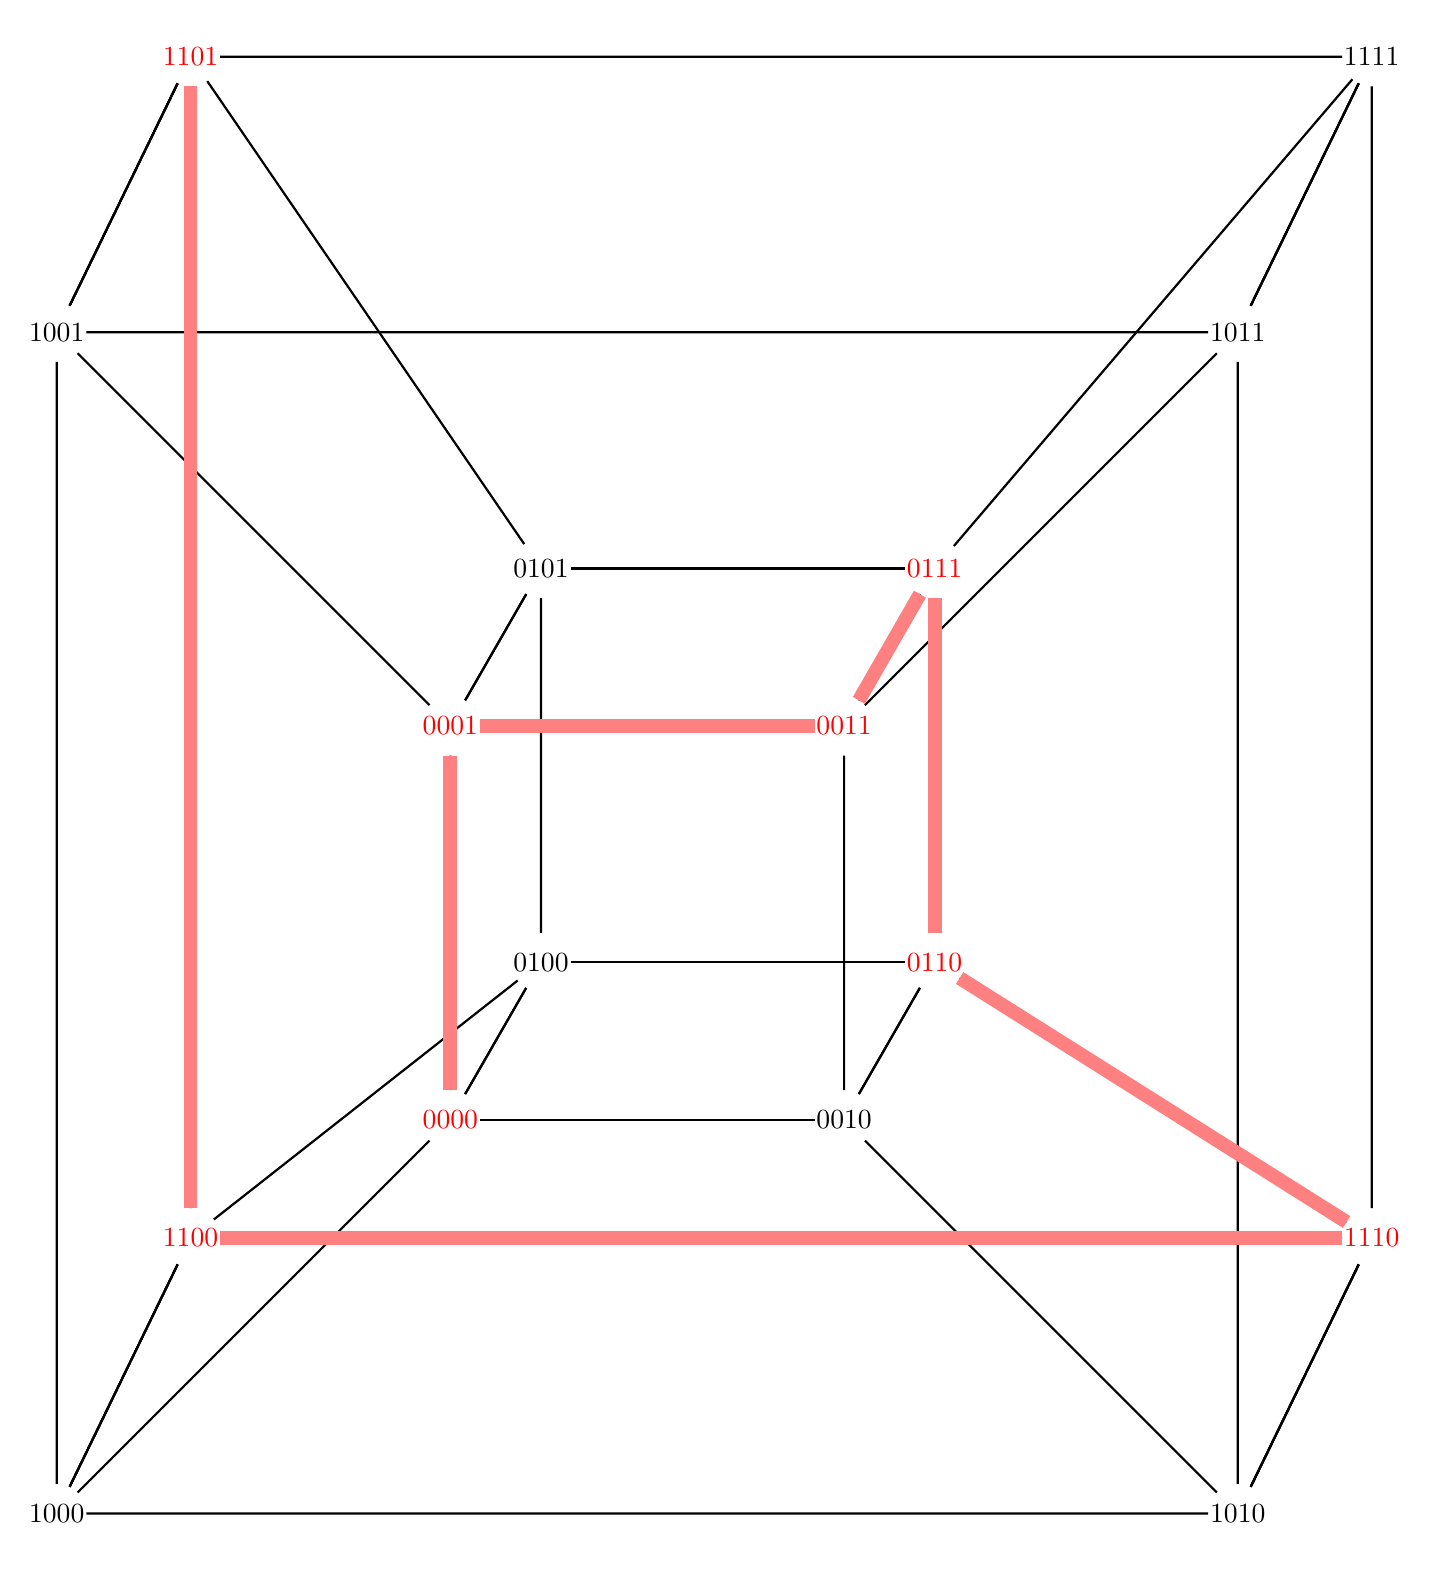
\begin{tikzpicture}[scale=5]
	 \tikzstyle{vertex}=[circle,minimum size=20pt,inner sep=0pt]
	 \tikzstyle{selected vertex} = [vertex, fill=red!24]
	 \tikzstyle{selected edge} = [draw,line width=5pt,-,red!50]
	 \tikzstyle{edge} = [draw,thick,-,black]
	 \node[vertex, text=red] (v0) at (0,0) {$0000$};
	 \node[vertex, text=red] (v1) at (0,1) {$0001$};
	 \node[vertex] (v2) at (1,0) {$0010$};
	 \node[vertex, text=red] (v3) at (1,1) {$0011$};
	 \node[vertex] (v4) at (0.23, 0.4) {$0100$};
	 \node[vertex] (v5) at (0.23,1.4) {$0101$};
	 \node[vertex, text=red] (v6) at (1.23,0.4) {$0110$};
	 \node[vertex, text=red] (v7) at (1.23,1.4) {$0111$};
	 \node[vertex] (v8) at (-1,-1) {$1000$};
	 \node[vertex] (v9) at (-1,2) {$1001$};
	 \node[vertex, text=red] (v13) at (-0.66,2.7) {$1101$};
	 \node[vertex, text=red] (v12) at (-0.66,-0.3) {$1100$};
	 \node[vertex] (v10) at (2,-1) {$1010$};
	 \node[vertex, text=red] (v14) at (2.34,-0.3) {$1110$};
	 \node[vertex] (v11) at (2,2) {$1011$};
	 \node[vertex] (v15) at (2.34,2.7) {$1111$};
	 \draw[edge] (v0) -- (v1) -- (v3) -- (v2) -- (v0);
	 \draw[edge] (v0) -- (v4) -- (v5) -- (v1) -- (v0);
	 \draw[edge] (v2) -- (v6) -- (v7) -- (v3) -- (v2);
	 \draw[edge] (v4) -- (v6) -- (v7) -- (v5) -- (v4);
	 \draw[edge] (v8) -- (v9) -- (v13) -- (v12) -- (v8);
	 \draw[edge] (v0) -- (v4) -- (v12) -- (v8) -- (v0);
	 \draw[edge] (v1) -- (v9) -- (v13) -- (v5) -- (v1);
	 \draw[edge] (v2) -- (v10) -- (v14) -- (v6) -- (v2);
	 \draw[edge] (v8) -- (v10) -- (v14) -- (v12) -- (v8);
	 \draw[edge] (v3) -- (v11) -- (v15) -- (v7) -- (v3);
	 \draw[edge] (v10) -- (v11) -- (v15) -- (v14) -- (v10);
	 \draw[edge] (v9) -- (v11) -- (v15) -- (v13) -- (v9);
	 \draw[selected edge] (v0) -- (v1);
	 \draw[selected edge] (v1) -- (v3);
	 \draw[selected edge] (v3) -- (v7);
	 \draw[selected edge] (v7) -- (v6);
	 \draw[selected edge] (v6) -- (v14);
	 \draw[selected edge] (v14) -- (v12);
	 \draw[selected edge] (v12) -- (v13);
	 %\draw[selected edge] (v14) -- (v15);
	 %\draw[selected edge] (v15) -- (v7);
	 %\draw[selected edge] (v7) -- (v3);
	 %\draw[selected edge] (v3) -- (v1);
	 %\draw[selected edge] (v1) -- (v9);
	 %\draw[selected edge] (v9) -- (v11);
	 %\draw[selected edge] (v11) -- (v10);
	 %\draw[selected edge] (v10) -- (v8);
	 %\draw[selected edge] (v8) -- (v0);
 \end{tikzpicture}
 }
 \end{figure}
\end{document}
\end{document}